\section{Methodology}
% \begin{figure*}[h]
% % \vspace{-2mm}
% \centering
% \includegraphics[width=16cm]{imgs/algo.png}
% \caption{Illustration of the proposed Asynchronous LinUCB Algorithm \textcolor{red}{make this diagram flatter? illustrate the second algorithm in this diagram as well?}}
% \label{fig:algo}
% % \vspace{-3mm}
% \end{figure*}
In this section, we establish the asynchronous event-triggered communication framework for federated linear bandit, and propose two UCB-type algorithms under different assumptions about the clients' reward functions, followed by our theoretical analysis of their regret and communication cost.
% In this section,  we first formulate the problem studied in this paper. Then we identify the connection between regret and communication cost for federated linear bandit algorithms, and establish the asynchronous event-triggered communication framework to balance these two objectives. Based on the communication framework, we propose two upper confidence bound algorithms under different assumptions about the reward functions among the clients, followed by our theoretical analysis of their regret and communication cost.

\subsection{Problem Formulation} \label{subsec:problem_formulation}
Consider a learning system with 1) $N$ clients responsible for taking actions and receiving reward feedback from the environment, e.g., each client being an edge device directly interacting with a user, and 2) a central server responsible for coordinating the communication between the clients for collaborative model estimation. 
% The clients can only communicate with the central server, instead of directly communicating with each other.
At each time $t=1,2,...,T$, an arbitrary client $i_{t} \in [N]$ (assume $P(i_{t}=i)>0,\forall i \in [N]$) interacts with the environment by choosing one of the $K$ actions, and receives the corresponding reward. When making the choice, client $i_{t}$ has access to a set $\cA_{t}=\{\bx_{t,1}, \bx_{t,2}, \dots, \bx_{t,K}\}$, where $\bx_{t, a}$ denotes the context vector associated with the $a$-th action for client $i_{t}$ at time $t$. Denote the context vector of the chosen action at time $t$ as $\bx_{t}$,
% an arm $a_{t}$ from a time-varying arm set $\cA_{t}=\{\bx_{t,1}, \bx_{t,2}, \dots, \bx_{t,|\cA_{t}|}\}$, where $\bx_{t, j}$ denotes the context vector associated with the $j$-th arm at time $t$. 
and the corresponding reward received by client $i_{t}$ as $y_{t}$, which is assumed to be generated by an unknown linear reward mapping $y_{t}=f_{i_{t}}(\bx_{t})+\eta_{t}$. As in standard linear bandit, $\eta_{t}$ is zero mean $\sigma$-sub-Gaussian noise conditioning on the $\sigma$-algebra generated by the previously pulled arms and the observed rewards $\cF_{t-1}=\sigma\{\bx_{1},y_{1},\bx_{2},y_{2},\dots,\bx_{t-1},y_{t-1},\bx_{t}\}$. Interaction between the learning system and the environment repeats itself, and the goal of the learning system is to minimize the accumulative (pseudo) regret $R_{T}=\sum_{t=1}^{T}r_{t}$ where $r_{t}=\max_{\bx \in \cA_{t}}f_{i_{t}}(\bx)-f_{i_{t}}(\bx_{t})$. 
% \chuanhao{Does the new assumption require us to change the definition of regret here, i.e., expectation over context as well? It seems not.}

\begin{figure}[t]
% \vspace{-4mm}
\centering
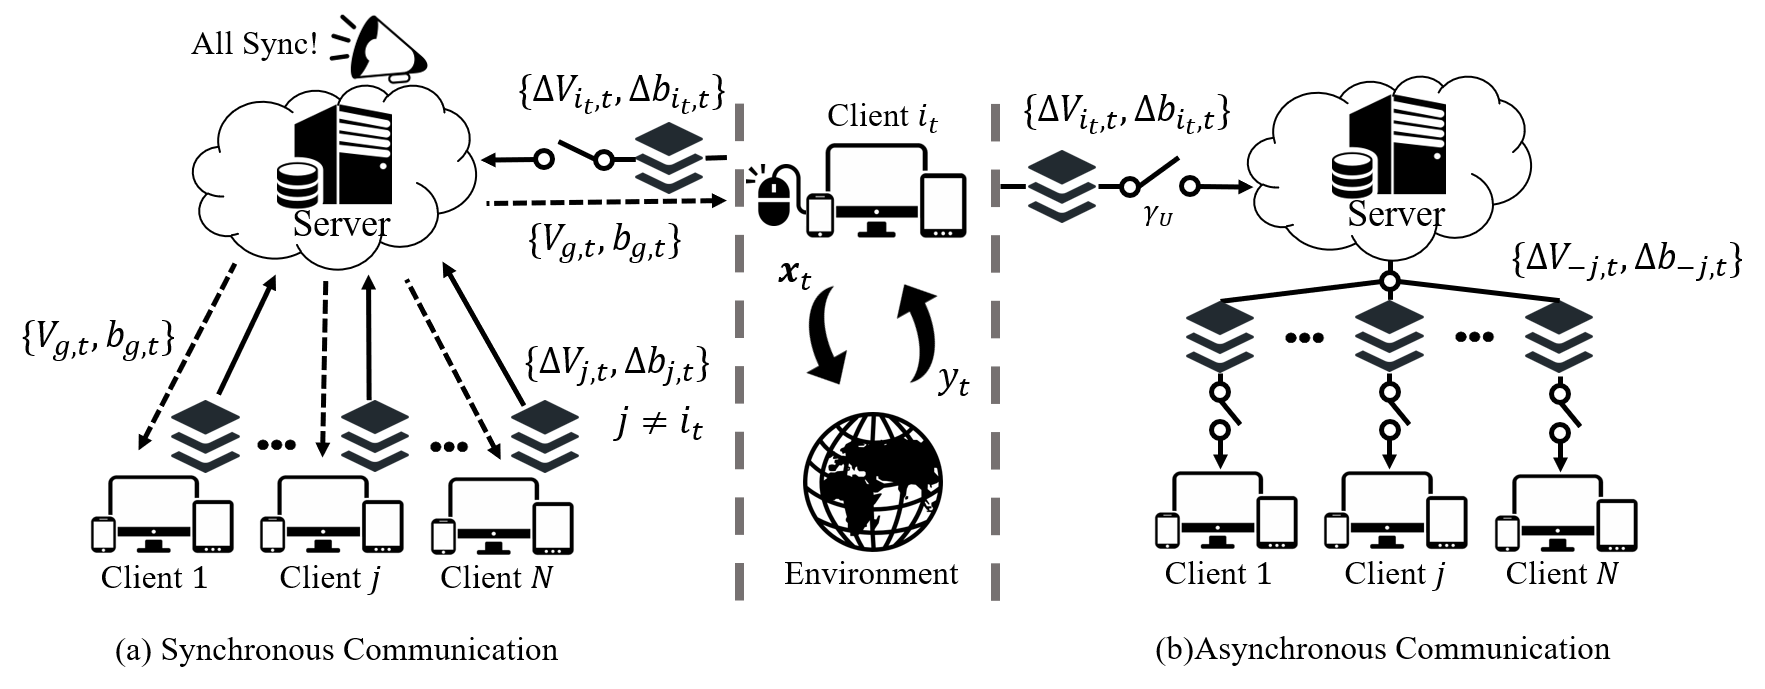
\includegraphics[width=14cm]{imgs/sync_vs_async.png}
% \vspace{-3mm}
\caption{Comparison between the synchronous and asynchronous event-triggered communications for federated linear bandit. The former requires all clients to upload their latest data at once and then download the aggregated data, while latter performs both upload and download on a per-client basis.}
\label{fig:algo}
% \vspace{-1mm}
\end{figure}

Denote the set of time steps when client $i$ interacts with the environment up to time $t$ as $\cN_{i}(t)=\left\{1 \leq \tau \leq t:i_{\tau}=i\right\}$. Note that we do not impose any further assumption on the clients' distribution or frequency of its interactions. This makes our setting more general than existing works \citep{wang2019distributed,dubey2020differentially}, where the clients interact with the environment in a round-robin fashion, i.e., $|\cN_{i}(t)|=t/N$. 
In addition, in the federated learning setting, the clients cannot directly communicate with each other, but can only communicate with the central server, i.e., a star-shaped communication network. Raw data collected by each client $\{(\bx_{\tau},y_{\tau})\}_{\tau \in \cN_{i}(t)}$ is stored locally and will not be transferred. Instead, the clients can only collaborate by communicating the parameters of the learning algorithm, e.g., gradients or sufficient statistics; and the communication cost is measured by the amount of parameters transferred across the system up to time $T$, which is denoted by $C_{T}$.
% Raw data sharing is also not allowed, and the clients can only collaborate by communicating the parameters of the learning algorithm, which in this paper, are just the sufficient statistics for the raw data, since analytical solution exists for linear bandit problem. And the communication cost is simply measured by the number of times data is transferred from one agent in the learning system (either client or server) to another.

We consider two different settings about the linear reward mapping function $f_{i}(\cdot)$ for $i=1,\dots,N$:

\paragraph{Homogeneous clients.}
Rewards received by all the clients are generated by a common reward mapping function:
    \begin{equation}\label{eq:homo_theta}
        f_{i}(\bx)=\theta^{\top} \bx, \quad \forall i \in [N]
    \end{equation}
    where $\theta \in \bR^{d}$ is the unknown parameter and we assume $\lVert \theta\rVert \leq 1$ and $\lVert \bx \rVert \leq 1$. Despite its simplicity, this setting is commonly adopted in existing works for federated bandits.
    % , which we refer to as homogeneous clients.
\paragraph{Heterogeneous clients.}
The unknown parameter for each client $i\in [N]$ consists of a globally shared component $\theta^{(g)}\in \bR^{d_{g}}$ and a unique local component $\theta^{(i)}\in \bR^{d_{i}}$: 
    \begin{equation}\label{eq:hetero_theta}
        f_{i}(\bx)= \begin{bmatrix} \theta^{(g)} \\ \theta^{(i)} \end{bmatrix}^{\top} \begin{bmatrix} \bx^{(g)} \\ \bx^{(l)} \end{bmatrix} , \quad \forall i \in [N]
    \end{equation}
    where $\bx^{(g)}\in \bR^{d_{g}}$, $\bx^{(l)}\in \bR^{d_{i}}$ denote the global and local features in $\bx$, and we assume $||\theta^{(g)}||_{2} \leq 1$, $||\theta^{(i)}||_{2} \leq 1, \forall i\in [N]$ and $||\bx^{(g)}||_{2} \leq 1$, $||\bx^{(l)}||_{2} \leq 1$. 
    This setting is more general and fits a larger variety of problems in practice. For example, $\bx^{(g)}$ could be common arm features relevant to all the clients and $\bx^{(l)}$ are those unique to client $i$. And our setting is flexible enough to allow different clients to have varying dimensions of their local features (i.e., $d_{i}\ne d_j$). Alternatively, when $\bx^{(g)}\equiv\bx^{(l)}$, this recovers the multi-task learning setting in \cite{evgeniou2004regularized}. 
    % We refer to this setting as heterogeneous clients, and 

We adopt the context regularity assumption from \cite{gentile2014online,li2019improved,li2021unifying}, which imposes a variance condition on the stochastic process generating $\bx_{t,a}$ (for heterogeneous clients, it is imposed on global features $\bx_{t,a}^{(g)}$). This suggests the informativeness of each observation in expectation. 
% In practice, it means each arm has diverse features over time.
% In practice, it means each arm has diverse features over time, i.e., possible values of $\bx_{t,a}$ for each $a \in [K]$ span $\bR^{d}$. This is slightly stronger than the common assumption that the possible values of $\{\bx_{t,a}\}_{a\in [K]}$ together span $\bR^{d}$.
% But we will see that this assumption does give existing methods \cite{wang2019distributed} any advantage.
% \begin{assumption}[Context regularity] \label{assump:context_diversity}
% At each time $t$, the context vector $\bx_{t,a} \in \cA_{t}$ for each arm $a\in [K]$ is independently generated from a random process, such that $\bE_{t-1}[\bx_{t,a}\bx_{t,a}^{\top}] := \bE[\bx_{t,a}\bx_{t,a}^{\top}|\{i_{s},\cA_{s},\eta_{s}\}_{s\in [t-1]}] =\Sigma_{c} \succeq \lambda_{c} I, \forall t\in [T]$,
% % \begin{align*}
% %     & \bE_{t-1}[\bx_{t,a}\bx_{t,a}^{\top}] := \bE[\bx_{t,a}\bx_{t,a}^{\top}|\{i_{s},\cA_{s},\eta_{s}\}_{s\in [t-1]}] \\
% %     & =\Sigma_{c} \succeq \lambda_{c} I, \forall t\in [T]
% % \end{align*}
% where the constant $\lambda_{x} > 0$.
% % s
% % $\forall a \in [K], \bE_{t-1}[\bx_{t,a} \bx_{t,a}^{\top}]=\bE[\bx_{t,a} \bx_{t,a}^{\top}|\{\eta_{},\bx_{t,a}\}] =\Sigma_{x} \geq \lambda_{min} I$, or equivalently $\text{span}\{\bx_{t,a}|\bx_{t,a} \in \cX_{i_{t}}, i \in [N] \}=\bR^{d}$.
% % $\bE_{t-1}[\bx_{t,a} \bx_{t,a}^{\top}]=\bE[\bx_{t,a} \bx_{t,a}^{\top}|\{\eta_{},\bx_{t,a}\}]$
% \end{assumption}
\begin{assumption}[Context regularity] \label{assump:context_diversity}
At each time $t$, the context vector $\bx_{t,a} \in \cA_{t}$ for each arm $a\in [K]$ is independently generated from a random process, such that $$\bE_{t-1}[\bx_{t,a}\bx_{t,a}^{\top}] := \bE[\bx_{t,a}\bx_{t,a}^{\top}|\{i_{s},\cA_{s},\eta_{s}\}_{s\in [t-1]}] =\Sigma_{c} \succeq \lambda_{c} I, \forall t\in [T]$$ where the constant $\lambda_{c} > 0$. Let also, for any fixed unit vector $z \in \bR^{d}$, the random variable $(z^{\top} \bx_{t,a})^{2}$ be conditionally sub-Gaussian with variance parameter $v^{2} \leq {\lambda_{c}^{2}}/{(8\log{4K})}$.
\end{assumption}
% \chuanhao{The ``collective diversity" assumption is enough to show $\lambda_{min}(V_{t-1})=\Omega(t)$, since each client has a non-zero probability to show up so that the span of the context vector at any time is $\bR^{d}$, and a standard construction of matrix martingale and application of the Freedman inequality can do the job. The main problem is with $\lambda_{min}(V_{i,t-1})$ (this is what we need), which is decided by both the environment and the algorithm, i.e., the algorithm is essentially picking a subset of the data in $V_{t-1}$ to construct $V_{i,t-1}$, and our fear is that after this ``picking", the data point in the resulting matrix no longer satisfies the condition. If this ``picking" is conducted such that each element in $V_{t-1}$ has none zero probability to be picked, then it seems to be fine.}

% \chuanhao{conditioning on history, there are two source of randomness, user showing up at time t and context vector drawn from the distribution of this user at time t}

% \textcolor{blue}{Do we need discussions about these two settings? e.g. setting 1 is the same as existing works, and setting 2 has a multi-task learning flavor which can be beneficial for some cases}

% The rewards observed by all the clients are generated by the same reward mapping function parameterized by an unknown bandit parameter $\theta$ (assume $\lVert \theta\rVert \leq S$). Under this assumption, reward at time $t$ is $y_{t} = \bx_{t}^\top \theta+\eta_{t}$, where $\eta_{t}$ is assumed to be $\sigma$-sub-gaussian conditioning on the $\sigma$-algebra generated by the pulled arms and the observed rewards $\cF_{t-1}=\sigma\{X_{1},Y_{1},X_{2},Y_{2},\dots,X_{t-1},Y_{t-1},X_{t}\}$. 

% the reward observed by client $i_t$ is generated by $y_{t}=[{\bx^{(g)}_{t}}^{\top},  {\bx^{(l)}_{t}}^{\top}] \begin{bmatrix} \theta^{(g)} \\ \theta^{(i_{t})} \end{bmatrix} + \eta_{t}$, where $\theta^{(g)} \in \bR^{d_{g}}$, $\theta^{(i_{t})} \in \bR^{d_{l}}$ denote the global bandit parameter and client $i_{t}$'s local bandit parameter respectively, and $\bx^{(g)}_{t}\in \bR^{d_{g}}$, $\bx^{(l)}_{t}\in \bR^{d_{l}}$ denote the components of context vector $\bx_{t}$ corresponding to the global and local bandit parameters. We also assume that $||\theta^{(g)}||_{2} \leq S_{g}$, $||\theta^{(i)}||_{2} \leq S_{l}, \forall i\in [N]$ and $||\bx^{(g)}||_{2} \leq L_{g}$, $||\bx^{(l)}||_{2} \leq L_{l}$.


\subsection{Asynchronous Communication Framework}\label{subsec:async_comm}
In order to balance the two conflicting objectives, i.e., regret $R_{T}$ and communication cost $C_{T}$, we introduce an asynchronous event-triggered communication framework as illustrated in Figure \ref{fig:algo}(b). For simplicity, all discussions in this section assume homogeneous clients (Eq \eqref{eq:homo_theta}), and we show in Section \ref{subsec:async_LinUCB_AM} that the result extends to heterogeneous clients (Eq \eqref{eq:hetero_theta}) as well with minor modifications. Also note that in this paper we use LinUCB \citep{abbasi2011improved} with our communication framework as a running example, but our results readily hold for other popular algorithms like LinTS \citep{abeille2017linear} and LinPHE \citep{kveton2019perturbed}  \footnote{Their regret bounds also depend on $\sum_{t=1}^{T}\lVert \bx_{t} \rVert_{V_{t-1}^{-1}}$ (see $R_{\text{TS}}(T)$ in Section 4 of \citet{abeille2017linear} and Theorem 1 in \citet{kveton2019perturbed}). Therefore a similar procedure can be applied, i.e., plug our Algorithm \ref{algo:comm} into LinTS to communicate the $V$ matrix, or into LinPHE to communicate the unperturbed $G$ matrix.}.

We begin our discussion with an important observation about the instantaneous regret of linear bandit algorithms.
% \cite{abbasi2011improved,abeille2017linear,kveton2019perturbed}.
% The design of our asynchronous event-triggered communication framework is based on the following observation.
Denote the sufficient statistics (for $\theta$) collected from all clients by time $t$ as ${V}_{t}=\sum_{\tau=1}^{t}\bx_{\tau}\bx_{\tau}^{\top}$ and ${b}_{t}=\sum_{\tau=1}^{t}\bx_{\tau}y_{\tau}$. In a centralized setting, at each time step $t\in[T]$, $\{{V}_{t-1},{b}_{t-1}\}$ are readily available to make an informed choice of arm $\bx_{t}\in\cA_{t}$. It is known that the instantaneous regret $r_{t}$ incurred by the mentioned linear bandit algorithms is directly related to the width of the confidence ellipsoid in the direction of $\bx_{t}$. Specifically, from Theorem 3 in \citep{abbasi2011improved}, with probability at least $1-\delta$, the instantaneous regret $r_{t}$ incurred by LinUCB can be upper bounded by $r_{t}  \leq 2 \alpha_{t-1} \sqrt{\bx_{t}^{\top}V_{t-1}^{-1}\bx_{t}} $, where $\alpha_{t-1}=O\left(\sqrt{d\log{\frac{T}{\delta}}}\right)$.
% \textcolor{blue}{we can mention this framwork is general because regret analysis of most linear bandit algorithms rely on diameter of the ellipsoid? so similar procedure should still work for other algos, like LinTS?}
%\begin{align*}
%    r_{t} & \leq O\left(\sqrt{d\log{\frac{T}{\delta}}}\right) \sqrt{\bx_{t}^{\top}V_{t-1}^{-1}\bx_{t}} 
%\end{align*}
However, as data is decentralized in our problem, $\{{V}_{t-1},{b}_{t-1}\}$ are not readily available to client $i_{t}$. Instead, the client only has a delayed copy, denoted by  $\{{V}_{i_{t},t-1},{b}_{i_{t},t-1}\}$, which is obtained by its own interactions with the environment on top of the last communication with the server. Therefore, now the instantaneous regret $r_{t} \leq  2 \alpha_{i_{t},t-1} \sqrt{\bx_{t}^{\top}V_{i_{t},t-1}^{-1}\bx_{t}} = 2 \alpha_{i_{t},t-1} \sqrt{\bx_{t}^{\top}{V}_{t-1}^{-1}\bx_{t}}\sqrt{\Gamma_{t-1}}$, where $\Gamma_{t-1} =\frac{\bx_{t}^{\top}{V}_{i_{t},t-1}^{-1}\bx_{t}}{\bx_{t}^{\top}{V}_{t-1}^{-1}\bx_{t}}$ measures how much wider the confidence ellipsoid at client $i_{t}$'s estimation in the direction of $\bx_{t}$ is, compared with that under a centralized setting. The value of $\Gamma_{t-1}$ depends on how frequent local updates are aggregated and shared via the server. Also note that $\Gamma_{t-1} \geq 1$, as ${V}_{t-1} \succeq {V}_{i_{t},t-1},\forall t$, which suggests the regret in the decentralized setting is at best the same as that in the centralized setting. Equality is attained when all the clients are synchronized in every time step.

Based on this observation, we can balance regret and communication cost by controlling the value of $\Gamma_{t-1}$. 
However, in the decentralized setting, neither the server nor the clients has direct access to $\{V_{t-1},b_{t-1}\}$, and the closest thing one can get is the aggregated sufficient statistics managed by the server, which we denote as $\{V_{g,t-1},b_{g,t-1}\}$. Hence, we take an indirect approach by first ensuring $\{V_{g,t-1},b_{g,t-1}\}$ do not deviate too much from $\{V_{t-1},b_{t-1}\}$, and then $\{V_{i,t-1},b_{i,t-1}\}$ do not deviate too much from $\{V_{g,t-1},b_{g,t-1}\}$ for each client $i\in [N]$. The former leads to the `upload' event, i.e., each client decides whether to upload independently, and the latter leads to the `download' event, i.e., the server decides whether to send its latest statistics to each client independently as well. 
% In comparison, in the existing method \cite{wang2019distributed,dubey2020differentially}, synchronous upload from all $N$ clients is triggered if any client in the learning system deviates too much from the last communicated data, and then the server will passively aggregate all the uploaded data and return it to all $N$ clients.

% we design the following asynchronous communication framework and triggering events (illustrated as switches in Figure \ref{fig:algo}) that will trigger `upload' and `download' communications, which makes sure $\Gamma_{t-1}$ is always bounded by a constant value given in Lemma \ref{lem:Gamma_upperbound}.

% To facilitate further discussion, we denote the sufficient statistics of client $i$'s locally stored data at time $t$ as $\tilde{V}_{i,t}=\sum_{n \in \cN_{i}(t)}\bx_{n}\bx_{n}^{\top}$ and $\tilde{b}_{i,t}=\sum_{n \in \cN_{i}(t)}\bx_{n}y_{n}$. Then the sufficient statistics of the aggregated data over all clients at time $t$ are denoted by $\tilde{V}_{t}=\sum_{i=1}^{N}\tilde{V}_{i,t}$ and $\tilde{b}_{t}=\sum_{i=1}^{N}\tilde{b}_{i,t}$. 
% In a centralized machine learning setting, when a client interacts with the environment at time $t$, $\tilde{V}_{t-1}$ and $\tilde{b}_{t-1}$ are readily available for model estimation and arm selection. However, in a federated learning setting, only $\tilde{V}_{i,t-1}$ and $\tilde{b}_{i,t-1}$ are stored locally by client $i$. To obtain the same accumulative regret up to time $T$, the federated linear bandits would incur $N \cdot T$ communication cost, i.e. synchronizing all $N$ clients in each time step, but this communication overhead is too large for most decentralized applications.

% at each time when a client obtains a new data point $(\bx_{t},y_{t})$, it needs to send the update to the sufficient statistics to the server and then the server needs to forward it to the other $N-1$ clients, which is huge communication overhead and impractical for most applications.
% so in order to make sure client $i$ also has access to $\sum_{j\neq i}\tilde{V}_{j,t-1}$ and $\sum_{j \neq i}\tilde{b}_{i,t-1}$

% Instead, we design an even-triggered `upload' communication that each client will independently decide when to send its latest sufficient statistics to the server. We denote the recently `uploaded' copy of each client's sufficient statistics as $\bar{V}_{i,t-1}$ and $\bar{b}_{i,t-1}$ for $i\in[N]$. Since `upload' communication will not happen in every time step, the uploaded copy will be delayed compared with the latest local copy and their difference is denoted by $\Delta V_{i,t}=\tilde{V}_{i,t}-\bar{V}_{i,t-1}$ and $\Delta b_{i,t}=\tilde{b}_{i,t}-\bar{b}_{i,t-1}$.

% The server will aggregate the uploaded sufficient statistics from all the clients, and then decide independently for each client $j$ when to send the aggregated sufficient statistics $\sum_{i \neq j} \bar{V}_{i,t}$ and $\sum_{i \neq j} \bar{b}_{i,t}$ to it. This decision again is based on a `download' triggering event. We denote the recently downloaded copy of the aggregated sufficient statistics to client $j$ as $\bar{V}_{-j,t-1}$ and $\bar{b}_{-j,t-1}$.

% the clients need to occasionally `upload' their local sufficient statistics to the server where they will get aggregated, so that those clients can `download' the aggregated sufficient statistics from the server later.
% At time step $t$, we denote the copy of sufficient statistics client $i$ has been `uploaded' to the server as $\bar{V}_{i,t-1}$ and $\bar{b}_{i,t-1}$, and the copy of sufficient statistics client $i$ has recently `downloaded' from the server as $\bar{V}_{-i,t-1}$ and $\bar{b}_{-i,t-1}$.
% the aggregated sufficient statistics stored at the server as $\bar{V}_{g,t-1}$ and $\bar{b}_{g,t-1}$.
% In addition to the locally stored $\tilde{V}_{i,t-1}$ and $\tilde{b}_{i,t-1}$, client $i$ also has access to the sufficient statistics that have been recently downloaded from the server denoted by $\bar{V}_{-i,t-1}$ and $\bar{b}_{-i,t-1}$.
% \setlength{\textfloatsep}{5mm}
% \setlength{\floatsep}{5mm}
In the proposed communication framework shown in Figure \ref{fig:algo}(b), each client $i\in[N]$ stores a local copy of its sufficient statistics $\{V_{i,t-1},b_{i,t-1}\}$, and also an `upload' buffer $\{\Delta V_{i,t-1},\Delta b_{i,t-1}\}$, i.e., client $i$'s local updates that have not been sent to the server. At each time step $t$, client $i_{t}\in [N]$ interacts with the environment, and updates $V_{i_{t},t}=V_{i_{t},t-1}+\bx_{t}\bx_{t}^{\top},b_{i_{t},t}=b_{i_{t},t-1}+\bx_{t}y_{t}$, $\Delta V_{i_{t},t}=\Delta V_{i_{t},t-1}+\bx_{t}\bx_{t}^{\top},\Delta b_{i_{t},t}=\Delta b_{i_{t},t-1}+\bx_{t}y_{t}$ with the new observation $(\bx_{t},y_{t})$. Then it starts executing 
% the communication protocol described in 
Algorithm \ref{algo:comm}, by first checking the following condition (line 2):
% First, it checks the following condition (line 2 in Algorithm \ref{algo:comm}):

\noindent \textbf{`Upload' event}: Client $i_{t}$ sends $\{\Delta V_{i_{t},t},\Delta b_{i_{t},t}\}$ to the server if event:
% \small
    \begin{equation}\label{eq:upload}
        \cU_{t}(\gamma_{U}) = \left\{\frac{\det(V_{i_{t},t})}{\det(V_{i_{t},t}-\Delta V_{i_{t},t})} > \gamma_{U} \right\}
    \end{equation}
% \normalsize
happens, and then sets $\Delta V_{i,t}=\textbf{0},\Delta b_{i,t}=\textbf{0}$. Otherwise, $\{\Delta V_{i,t}, \Delta b_{i,t}\}$ remain unchanged.

The server stores the aggregated sufficient statistics $\{V_{g,t-1},b_{g,t-1}\}$ over the local updates received from the clients, and also maintains `download' buffers $\{\Delta V_{-j,t-1},\Delta b_{-j,t-1}\}$ for each client $j\in [N]$, i.e., the aggregated updates that have not been sent to client $j$. Specifically, after the server receives $\{\Delta V_{i_{t},t},\Delta b_{i_{t},t}\}$ via the `upload' from client $i_t$, it updates $V_{g,t}=V_{g,t-1}+\Delta V_{i_{t},t},b_{g,t}=b_{g,t-1}+\Delta b_{i_{t},t}$, and $\Delta V_{-j,t}=\Delta V_{-j,t-1}+\Delta V_{i_{t},t},\Delta b_{-j,t}=\Delta b_{-j,t-1}+\Delta b_{i_{t},t}$ for all clients $j \neq i_{t}$. Then it checks the following condition for each client $j \neq i_{t}$ (line 7):

\noindent \textbf{`Download' event}: The server sends $\{\Delta V_{j,t},\Delta b_{j,t}\}$ to client $j$ if event:
% \small
    \begin{equation}\label{eq:download}
        \cD_{t,j}(\gamma_{D})=\left\{\frac{\det(V_{g.t})}{\det(V_{g,t}-\Delta V_{-j,t})} > \gamma_{D}\right\}
    \end{equation}
% \normalsize
happens, and then sets $\Delta V_{-j,t}=\textbf{0},\Delta b_{-j,t}=\textbf{0}$. Otherwise, $\{\Delta V_{-j,t}, \Delta b_{-j,t}\}$ remain unchanged.

After client $j$ receives $\{\Delta V_{-j,t},\Delta b_{-j,t}\}$ via the `download' communication, it updates $V_{j,t}=V_{j,t-1}+\Delta V_{-j,t},b_{j,t}=b_{j,t-1}+\Delta b_{-j,t}$.
% \begin{itemize}
%     \item `Upload': At time $t$, after client $i_{t}$ observes the new data point $(\bx_{t},y_{t})$ and locally updates $\tilde{V}_{i_{t},t}$ and $\tilde{b}_{i_{t},t}$, client $i_{t}$ will send $\tilde{V}_{i_{t},t}$ and $\tilde{b}_{i_{t},t}$ to the server if:
%     \begin{equation}\label{eq:upload}
%         \frac{\det(\tilde{V}_{i_{t},t}+\bar{V}_{-i_{t},t-1})}{\det(\bar{V}_{i_{t},t-1}+\bar{V}_{-i_{t},t-1})} \geq \gamma_{U}
%     \end{equation}
%     \item `Download': Upon receiving sufficient statistics from client $i_{t}$, the server will update its aggregated sufficient statistics accordingly. The server will then check the following condition for each client $j\neq i_{t}$, and send $\sum_{i \neq j} \bar{V}_{i,t}$ and $\sum_{i \neq j} \bar{b}_{i,t}$ to client $j$ if:
%     \begin{equation}\label{eq:download}
%         \frac{\det(\bar{V}_{j,t-1}+\sum_{i \neq j} \bar{V}_{i,t})}{\det(\bar{V}_{j,t-1}+\bar{V}_{-j,t-1})} \geq \gamma_{D}
%     \end{equation}
% \end{itemize}
\begin{algorithm}[h]
    \caption{Event-triggered Communication Protocol} \label{algo:comm}
  \begin{algorithmic}[1]
    \STATE \textbf{Input:} thresholds $\gamma_{U}, \gamma_{D} \geq 1$
        \IF{ Event $\cU_{t}(\gamma_{U})$ in Eq \eqref{eq:upload} happens}
            \STATE Upload $\Delta{V}_{i_{t},t},\Delta{b}_{i_{t},t}$ ($\text{client } i_{t} \rightarrow \text{server}$) 
            \STATE Update server:
            % $V_{g,t}=V_{g,t-1}+\Delta V_{i_{t},t},b_{g,t}=b_{g,t-1}+\Delta b_{i_{t},t}$ \newline
            % $\Delta V_{-j,t}=\Delta V_{-j,t-1}+\Delta V_{i_{t},t},\Delta b_{-j,t}=\Delta b_{-j,t-1}+\Delta b_{i_{t},t}$ for $j \neq i_{t}$
            $V_{g,t}\mathrel{+}=\Delta V_{i_{t},t},b_{g,t}\mathrel{+}=\Delta b_{i_{t},t}$, $\Delta V_{-j,t}\mathrel{+}=\Delta V_{i_{t},t},\Delta b_{-j,t}\mathrel{+}=\Delta b_{i_{t},t}$, $\forall j \neq i_{t}$
            \STATE Client $i_{t}$ sets $\Delta{V}_{i_{t},t}=\textbf{0}$, $\Delta{b}_{i_{t},t}=\textbf{0}$
            % and $j \neq i_{t}$
            \FOR{$j = 1, \dots, N$} 
                \IF{ Event $\cD_{t,j}(\gamma_{D})$ in Eq \eqref{eq:download} happens}
                    \STATE Download $\Delta{V}_{-j,t},\Delta{b}_{-j,t}$ ($\text{server} \rightarrow \text{client } j$)
                    \STATE Update client $j$:
                    % $V_{j,t}=V_{j,t-1}+\Delta V_{-j,t},b_{j,t}=b_{j,t-1}+\Delta b_{-j,t}$
                    $V_{j,t}\mathrel{+}=\Delta V_{-j,t},b_{j,t}\mathrel{+}=\Delta b_{-j,t}$
                    \STATE Server sets $\Delta{V}_{-j,t}=\textbf{0},\Delta{b}_{-j,t}=\textbf{0}$
                \ENDIF
            \ENDFOR
        % \ELSE
        %     \STATE All other sufficient statistics remain unchanged
        \ENDIF
  \end{algorithmic}
\end{algorithm}

The following lemma specifies an upper bound of $\Gamma_{t-1}$ by executing Algorithm \ref{algo:comm}, which depends on the thresholds $\{\gamma_{U}, \gamma_{D}\}$ and the number of clients $N$.
\begin{lemma}\label{lem:Gamma_upperbound}
Under Assumption \ref{assump:context_diversity}, the `upload' and `download' triggering events defined in Eq \eqref{eq:upload} and Eq \eqref{eq:download}, then w.h.p. $\Gamma_{t-1} \leq \frac{8\gamma_{D}}{\lambda_{c}} [1+(N-1)(\gamma_{U}-1)],\forall t$.
\end{lemma}

Proof of Lemma \ref{lem:Gamma_upperbound} is given in appendix. The main idea is to use $\det(V_{g,t-1})$ as an intermediate between $\det(V_{i_{t},t-1})$ and $\det(V_{t-1})$, which are separately controlled by the `download' and `upload' events. When setting $\gamma_{D}=\gamma_{U}=1$, $\Gamma_{t-1}=1$, $\forall t \in [T]$, which means global synchronization happens at each time step, it recovers the regret incurred in the centralized setting.

% \begin{remark}[Synchronous vs. asynchronous communication] 
\noindent \textbf{Synchronous vs. asynchronous communication:}
%As illustrated in Figure \ref{fig:algo}, both the synchronous communication from \cite{wang2019distributed,dubey2020differentially} and the proposed asynchronous communication are event-triggered. 
% (based on determinant of covariance matrix). 
%In the former, 
As shown in Figure \ref{fig:algo}(a), in the synchronous protocol (Appendix G in \citep{wang2019distributed}), when a synchronization round is triggered by a client $i_{t}$, the server asks \emph{all} the clients to upload their local updates (illustrated as solid lines), aggregates them, and then sends the aggregated update back (illustrated as dashed lines). This `two-way' communication is vulnerable to delays or unavailability of clients, which are common in a distributed setting.
In comparison, our asynchronous communication, as shown in Figure \ref{fig:algo}(b), is more robust because the server only concerns the clients whose `download' condition has been met, which does not need other clients' acknowledgement. 
In addition, when the clients have distinct availability of new observations, which is usually the case for most applications, synchronizing all $N$ clients leads to inefficient communication as some clients may have very few new observations since last synchronization. We will show later that this unfortunately leads to an increased rate in $N$ in the upper bound of $C_{T}$, compared with our asynchronous communication.
% In addition, global synchronization requires every client in the learning system to send its local update despite the53fact some clients have very few new observations since last synchronization.
% In comparison, in the existing method \cite{wang2019distributed,dubey2020differentially}, synchronous upload from all $N$ clients is triggered if any client in the learning system deviates too much from the last communicated data, and then the server will passively aggregate all the uploaded data and return it to all $N$ clients.
% \end{remark}
% For example, when some client $j$ is temporarily unavailable to receive `download' communication or the packet is lost, the learning system can proceed to next round of interaction as usual, with the server trying to re-send the update in the background. As long as client $j$ receives the update before it interacts with the environment next time, the upper bound of $\Gamma_{t-1}$ in Lemma \ref{lem:Gamma_upperbound} always holds.

% \begin{remark}[Multiple Clients per Time Step]
\noindent \textbf{Multiple clients per time:}
Note that essentially both Algorithm \ref{algo:comm} and the synchronous protocol assumed only one active client per time, i.e., the communication protocol is executed after the current client receives a new observation and completed \textit{before} the next client shows up. 
This setup simplifies the description and also makes the theoretical results compatible with standard linear bandit setting. Otherwise, we will need to introduce additional assumptions to quantify the extent of delay in the communication for regret analysis.
In reality, each client is an independent process interacting with its environment, e.g., serving its user population, so that there could be many active clients at the same time. In the proposed asynchronous protocol, when a client triggers the upload event, it will immediately send the data in its buffer to the server; the server, upon receiving the uploaded data from any client, will immediately aggregate this data and check the download events to see which client needs a download. Thus, different from the synchronous protocol where the server ensures all the clients have the same model after each download, we allow both the server and the clients to update their model at any time without the need of any global synchronization.

% In a setting with multiple active clients per time, i.e., the communication protocol is only executed after multiple clients have obtained new observations, Algorithm \ref{algo:comm} still applies with a minor modification: simultaneously, each active client checks their `upload' condition and sends local updates when needed, such that the server can aggregate local updates from multiple clients before checking the `download' condition. Lemma \ref{lem:Gamma_upperbound} can be readily adapted to account for the delay in processing the new observations obtained by clients that show up simultaneously in this time step.

% We assumed only one client interacts with the environment at each time step
% However, with minor modifications, Algorithm \ref{algo:comm} and the result in Lemma \ref{lem:Gamma_upperbound} apply to the setting where an arbitrary subset of clients are active at the same time: simultaneously, each active client checks their `upload' condition and sends communications when needed, such that the server can aggregate local updates from multiple clients before checking the `download' condition.
% \end{remark}

% \begin{remark}
% \textbf{Opportunity to further reduce `download' communication:}
% A design choice made in Algorithm \ref{algo:comm} is that the server always checks the `download' condition for every client even if some clients may not be active in the near future. This is because the server cannot predict when a client will be active, and has to ensure all clients are `up-to-date' all the time. For example, existing works assume all clients interact with the environment in a round-robin fashion \cite{wang2019distributed,dubey2020differentially}.
% In applications where the server gets informed about when a client will be active (e.g., via a pull request), it is much more communication-efficient for the server to only send aggregated updates to those clients by then, and keep updating the `download' buffer otherwise.

% An implicit assumption behind the current design is that sending data to a client right before it takes an action is not allowed. For example, a mobile app needs to be responsive when user opens it, instead of having to merge an update first. And because the learning system cannot predict which client will be active next time, it needs to ensure all the clients are `up-to-date' by checking their `download' triggering events (line 6 in Algorithm \ref{algo:comm}). Otherwise, for applications without this constraint, the server still updates the `download' buffer for each client in the same way, but only sends aggregated update to the client who is going to take an action next, which will make the communication more efficient.
% \end{remark}


%\subsection{Asynchronous LinUCB Algorithm}
\subsection{Learning with Homogeneous Clients}
\label{subsec:async_LinUCB}
Based on the asynchronous event-triggered communication, we design the Asynchronous LinUCB Algorithm (\modelone{}) for homogeneous clients. Detailed steps are explained in Algorithm \ref{algo:AsyncLinUCB}.

\noindent \textbf{Arm selection}:
At each time step $t=1,\dots,T$, 
% when client $i_{t}\in[N]$ interacts with the environment, 
% it has access to sufficient statistics of its local data $\tilde{V}_{i_{t},t-1},\tilde{b}_{i_{t},t-1}$ and the aggregated sufficient statistics $\bar{V}_{-i_{t},t-1},\bar{b}_{-i_{t},t-1}$ recently downloaded from the server. 
client $i_{t}$ selects an arm $\bx_{t} \in \cA_{t}$ using the the UCB strategy. Specifically, client $i_{t}$ pulls arm $\bx_{t}$ that maximizes the UCB score computed as follows (line 8),
\begin{equation}\label{eq:UCB}
    \bx_{t}=\argmax_{\bx \in \cA_{t}}{\bx^{\top}\hat{\theta}_{i_{t},t-1}(\lambda)+\text{CB}_{i_{t},t-1}(\bx)}
\end{equation}
where $\hat{\theta}_{i_{t},t-1}(\lambda)= V_{i_{t},t-1}(\lambda)^{-1}b_{i_{t},t-1}$ is the ridge regression estimator with regularization parameter $\lambda$; $V_{i_{t},t-1}(\lambda)=V_{i_{t},t-1}+\lambda I$; and the confidence bound of reward estimation for arm $\bx$ is $\text{CB}_{i_{t},t-1}(\bx)=\alpha_{i_{t},t-1}||\bx||_{V_{i_{t},t-1}(\lambda)^{-1}}$, where 
$\alpha_{i_{t},t-1}=\sigma \sqrt{\log{\frac{\det{V_{i_{t},t-1}(\lambda) }}{\det{\lambda I}}}+2\log{1/\delta}}+\sqrt{\lambda}$.
% $\alpha_{i_{t},t-1}=\sigma\sqrt{d\log{(1+\frac{t-1}{d\lambda})} + 2\log{\frac{1}{\delta}}}+\sqrt{\lambda}S$.
% where $\hat{\theta}_{i_{t},t-1}= \bigl(\bar{V}_{i_{t},t-1}+\tilde{V}_{-i_{t},t-1}+\lambda I\bigr)^{-1}\bigl(\bar{b}_{i_{t},t-1}+\tilde{b}_{-i_{t},t-1}\bigr)$ is the ridge regression estimator; and the confidence bound of reward estimation for arm $\bx$ is $\text{CB}_{i_{t},t-1}(\bx)=\alpha_{i_{t},t-1}||\bx||_{(\tilde{V}_{i_{t},t-1}+\tilde{V}_{-i_{t},t-1}+\lambda I)^{-1}}$, where $\alpha_{i_{t},t-1}=\sigma\sqrt{d\log{(1+\frac{t-1}{d\lambda})} + 2\log{\frac{1}{\delta}}}+\sqrt{\lambda}S$.
After client $i_{t}$ observes reward $y_{t}$ and updates locally (line 9), it proceeds with the asynchronous event-triggered communication (line 10), and sends updates accordingly.

% \setlength{\textfloatsep}{10mm}
\begin{algorithm}[h]
    \caption{\modelone{}} \label{algo:AsyncLinUCB}
  \begin{algorithmic}[1]
    \STATE \textbf{Input:} thresholds $\gamma_{U}, \gamma_{D} \geq 1$, $\sigma, \lambda > 0$, $\delta \in (0,1)$
    \STATE Initialize server: ${V}_{g, 0}=\textbf{0}_{d,d}$, ${b}_{g,0}=\textbf{0}_{d}$
        % \hspace*{2em} $\Delta{V}_{-i, 0}=\textbf{0} \in \mathbb{R}^{d \times d}$, $\Delta{b}_{-i,0}=\textbf{0} \in \mathbb{R}^{d}$, $i\in[N]$
    \FOR{ $t=1,2,...,T$}
        \STATE Observe arm set $\mathcal{A}_{t}$ for client $i_{t} \in [N]$
        \IF{client $i_{t}$ is new}
            \STATE Initialize client $i_{t}$: ${V}_{i_{t}, t-1}=\textbf{0}_{d,d}$, ${b}_{i_{t},t-1}=\textbf{0}_{d}$, $\Delta{V}_{i_{t}, t-1}=\textbf{0}_{d,d} $, $\Delta{b}_{i_{t},t-1}=\textbf{0}_{d}$
            \STATE Initialize server's download buffer for client $i_{t}$: $\Delta{V}_{-i_{t}, t-1}=V_{g,t-1}$, $\Delta{b}_{-i_{t},t-1}=b_{g,t-1}$
        \ENDIF
        \STATE Select arm $\bx_{t}\in\cA_{t}$ by Eq \eqref{eq:UCB} and observe reward $y_{t}$
        \STATE Update client $i_{t}$:
            % ${V}_{i_{t},t}={V}_{i_{t},t-1}+x_{t}x_{t}^{T}$, ${b}_{i_{t},t}={b}_{i_{t},t-1}+x_{t}y_{t}$ \newline
            % $\Delta{V}_{i_{t},t}=\Delta{V}_{i_{t},t-1}+x_{t}x_{t}^{T}$, $\Delta{b}_{i_{t},t}=\Delta{b}_{i_{t},t-1}+x_{t}y_{t}$
            ${V}_{i_{t},t} \mathrel{+}= \bx_{t}\bx_{t}^{T}$, ${b}_{i_{t},t} \mathrel{+}= \bx_{t}y_{t}$, $\Delta{V}_{i_{t},t} \mathrel{+}= \bx_{t}\bx_{t}^{T}$, $\Delta{b}_{i_{t},t}+=\bx_{t}y_{t}$
        \STATE Event-triggered Communications (Algorithm \ref{algo:comm})
        % \IF{ Event $\cU_{t}(\gamma_{U})$ (Eq \eqref{eq:upload}) happens}
        %     \STATE Upload $\Delta{V}_{i_{t},t},\Delta{b}_{i_{t},t}$ ($i_{t} \rightarrow \text{server}$) 
        %     \STATE Update server: \newline
        %     % $V_{g,t}=V_{g,t-1}+\Delta V_{i_{t},t},b_{g,t}=b_{g,t-1}+\Delta b_{i_{t},t}$ \newline
        %     % $\Delta V_{-j,t}=\Delta V_{-j,t-1}+\Delta V_{i_{t},t},\Delta b_{-j,t}=\Delta b_{-j,t-1}+\Delta b_{i_{t},t}$ for $j \neq i_{t}$
        %     \hspace*{1em} $V_{g,t}\mathrel{+}=\Delta V_{i_{t},t},b_{g,t}\mathrel{+}=\Delta b_{i_{t},t}$ \newline
        %     \hspace*{1em} $\Delta V_{-j,t}\mathrel{+}=\Delta V_{i_{t},t},\Delta b_{-j,t}\mathrel{+}=\Delta b_{i_{t},t}$, $j \neq i_{t}$
        %     \STATE Client $i_{t}$ reset $\Delta{V}_{i_{t},t}=\textbf{0}$, $\Delta{b}_{i_{t},t}=\textbf{0}$

        %     \FOR{$j = 1, \dots, N$ and $j \neq i_{t}$}
        %         \IF{ Event $\cD_{t,j}(\gamma_{D})$ (Eq \eqref{eq:download}) happens}
        %             \STATE Download $\Delta{V}_{-j,t},\Delta{b}_{-j,t}$ ($\text{server} \rightarrow j$)
        %             \STATE Update client $j$: \newline
        %             % $V_{j,t}=V_{j,t-1}+\Delta V_{-j,t},b_{j,t}=b_{j,t-1}+\Delta b_{-j,t}$
        %             \hspace*{1em} $V_{j,t}\mathrel{+}=\Delta V_{-j,t},b_{j,t}\mathrel{+}=\Delta b_{-j,t}$
        %             \STATE Server reset $\Delta{V}_{-j,t}=\textbf{0},\Delta{b}_{-j,t}=\textbf{0}$
        %         \ENDIF
        %     \ENDFOR
        % % \ELSE
        % %     \STATE All other sufficient statistics remain unchanged
        % \ENDIF
    \ENDFOR
  \end{algorithmic}
\end{algorithm}
% \setlength{\floatsep}{10mm}

% Then after client $i_{t}$ observes reward $y_{t}$ and updates its local sufficient statistics (line 6 in Algorithm 1), \modelone{} will check if the `upload' triggering event $\cU_{t}(\Gamma_{U})$ happens (line 7 in Algorithm 1), i.e. whether the sufficient statistics of client $i_{t}$ has varied much since its recent communication with the server due to local updates. If the `upload' communication is triggered, then client $i_{t}$ will send $\tilde{V}_{i_{t},t-1},\tilde{b}_{i_{t},t-1}$ to the server (line 8 in Algorithm 1).

% The server will update its aggregated sufficient statistics $\sum_{i=1}^{N}\bar{V}_{i,t},\sum_{i=1}^{N}\bar{b}_{i,t}$ after receiving client $i_{t}$'s uploaded sufficient statistics. Then it will check for each client $j \neq i_{t}$ if the `download' triggering event $\cD_{t,j}(\Gamma_{D})$ happens, i.e. whether the aggregated sufficient statistics stored on the server has varied much since its recent communication with client $j$ due to the newly uploaded sufficient statistics it receives from other clients (line 10 in Algorithm 1). If the `download' communication for client $j$ is triggered, then the server will send $\sum_{i\neq j}\bar{V}_{j,t},\sum_{i\neq j}\bar{b}_{j,t}$ to client $j$ (line 11 in Algorithm 1).

% The event-triggered communication framework introduced in Section \ref{subsec:comm_protocol} guarantees that at any time $t$, the sufficient statistics available to client $i_{t}$ are not too `delayed' (see Lemma \ref{lem:Gamma_upperbound}).

% \subsection{Regret and Communication Cost Analysis for \modelone{}} \label{subsec:regret_homo}
% \paragraph{Regret for \modelone{}}
The upper bounds of cumulative regret $R_{T}$ and communication cost $C_{T}$ incurred by \modelone{} are given in Theorem \ref{thm:regret_communication_async-linucb} (proof provided in appendix). Note that as discussed in Section \ref{subsec:async_comm}, clients collaborate by transferring updates of the sufficient statistics, i.e., $\{ \Delta V \in \bR^{d \times d},\Delta b \in \bR^{d}\}$. Since our target is not to reduce the size of these parameters, we define the communication cost $C_{T}$ as the number of times $\{ \Delta V,\Delta b\}$ being transferred between agents.
\begin{theorem}[Regret and Communication Cost] \label{thm:regret_communication_async-linucb}
With Assumption \ref{assump:context_diversity}, and the communication thresholds $\gamma_{U},\gamma_{D}$, then w.h.p., the cumulative regret $$R_{T} = O\left(d\sqrt{T\log^{2}{T}}\min(\sqrt{N},\sqrt{\gamma_{D} [1+(N-1)(\gamma_{U}-1)]})\right)$$ and communication $$C_{T} = O\bigl(d N {\log{T}}/{\log{\min{(\gamma_{U},\gamma_{D})}}}\bigr)$$
% $R_{T}$ has upper bound
% \small
% $$R_{T} = O\left(d\sqrt{T\log^{2}{T}}\min(\sqrt{N},\sqrt{\gamma_{D} [1+(N-1)(\gamma_{U}-1)]})\right)$$
% \normalsize
% The communication cost $C_{T}$ has upper bound
% $$C_{T} =\sum_{i=1}^{N} C_{T,i} \leq N \frac{\log{\det({V}_{T-1})}-d \log{\lambda}}{\log{\min{(\gamma_{U},\gamma_{D})}}}$$
\end{theorem}
The thresholds $\gamma_{U},\gamma_{D}$ can be flexibly adjusted to trade-off between $R_{T}$ and $C_{T}$, e.g., interpolate between the two extreme cases: clients never communicate ($R_{T}=O(N^{1/2}d\sqrt{T}\log{T})$); and clients are synchronized in every time step ($R_{T}=O(d\sqrt{T}\log{T})$). Details about threshold selection and the corresponding theoretical results are provided in appendix. For simplicity, we fix $\gamma_{U}=\gamma_{D}=\gamma$ in the following discussions, but one can choose different values to have a finer control especially for applications where the cost of upload and download communication differs. 
Based on Theorem \ref{thm:regret_communication_async-linucb}, to attain $R_{T}=O(N^{1/4}d\sqrt{T}\log{T})$, \modelone{} needs $C_{T}=O(N^{3/2}d\log{T})$ (by setting $\gamma=\exp(N^{-\frac{1}{2}})$). To attain the same $R_{T}$, the corresponding $C_{T}$ of \modelbaseline{} \footnote{\modelbaseline{} refers to DisLinUCB algorithm in Appendix G of \citep{wang2019distributed} adapted to our setting.} is smaller than ours by a factor of $O(N^{1/4})$ only under uniform client distribution ($P(i_{t}=i) = \frac{1}{N},\forall i\in[N]$), while under non-uniform client distribution, which is almost always the case in practice, it is higher than ours by a factor of $O(N^{1/4})$. The description and theoretical analysis of \modelbaseline{} under uniform and non-uniform client distribution are given in appendix.
% higher than ours by a factor of $O(N^{1/4})$ under non-uniform client distribution ($\exists i\in[N], P(i_{t}=i) \neq \frac{1}{N}$), and lower than ours by a factor of $O(N^{1/4})$ under uniform client distribution ($\forall i\in[N], P(i_{t}=i) = \frac{1}{N}$).
% Then if $\gamma= +\infty$, $C_{T}=0$ (no communication) and $R_{T}=O(N^{1/2}d \sqrt{T}\log{T})$. 
% As we mentioned earlier, the global synchronization of \modelbaseline{} is inefficient when the clients have different number of new observations, which is almost always the case in practice. For example, to attain $R_{T}=O(N^{1/4}d\sqrt{T}\log{T})$, \modelone{} needs $C_{T}=O(N^{3/2}d\log{T})$ (by setting $\gamma=\exp(N^{-\frac{1}{2}})$), 


% . We should note that the result of \modelone{} is agnostic to the client distribution. However, for the synchronous method \modelbaseline{}, 

% In addition, to compare with the existing synchronous solution \citep{wang2019distributed}, we adapt it to our problem setting and named the resulting algorithm \modelbaseline{} (the description and theoretical analysis of under uniform and non-uniform client distribution are given in appendix.).

% \begin{remark} \label{rmk:regret_comm}
% When $\gamma_{U}=\gamma_{D}= +\infty$, $C_{T}=0$ (no communication) and $R_{T}=O(N^{1/2}d \sqrt{T}\log{T})$. To get $R_{T}=O(N^{1/4}d\sqrt{T}\log{T})$, 
% % to reduce $R_{T}$ by a factor of $O(N^{1/4})$,
% \modelone{} needs $C_{T}=O(N^{3/2}d\log{T})$, which is better than \modelbaseline{} 
% \footnote{\modelbaseline{} refers to DisLinUCB in \cite{wang2019distributed}.
% % adapted to our setting.
% % , as they assumed clients show up in a round-robin fashion. 
% The description and theoretical analysis of this algorithm under uniform and non-uniform client distribution are given in appendix.} 
% by a factor of $O(N^{1/4})$ for non-uniformly sampled clients, but worse by a factor of $O(N^{1/4})$ for uniformly sampled clients.
% \end{remark}

% \begin{remark}\label{rmk:regret}
% The thresholds $\gamma_{U},\gamma_{D}$ can be flexibly adjusted to get various trade-off between $R_{T}$ and $C_{T}$. For simplicity, here we constrain $\gamma_{U}=\gamma_{D}=\gamma$, and summarize some choices of $\gamma$ and the corresponding results in Table \ref{tb:theoretical_comparison} (see detailed derivation in appendix), together with the results for \modelbaseline{} \footnote{\modelbaseline{} refers to the synchronous algorithm DisLinUCB in \cite{wang2019distributed} adapted to our setting, as they assumed clients show up in a round-robin fashion.
% For completeness, detailed description of \modelbaseline{} and theoretical analysis under both uniform and non-uniform client distributions are given in the appendix.}. We can see that \modelone{}'s result is not influenced by whether client distribution is uniform or not. In terms of $C_{T}$'s rate in $N$, it is slightly better than \modelbaseline{} under non-uniform distribution, and slightly worse than \modelbaseline{} under uniform distribution.

% \begin{table*}[h]
% \vspace{-4mm}
% \centering
% \caption{Upper bounds for $R_{T}$ and $C_{T}$ under different thresholds.}
% \begin{tabular}{ c c c c c}
% \toprule
% %  \multirow{2}{*}{Algorithm} & \multirow{2}{*}{Threshold} & \multirow{2}{*}{$R_{T}$} & \multicolumn{2}{c}{$C_{T}$} \\
% %  & & & uniform user & non-uniform user \\
%  Algorithm & Threshold & $R_{T}$ & $C_{T}$ (uniform) & $C_{T}$ (non-uniform) \\
%  \hline
%  \multirow{4}{*}{\modelone{}} 
%  & $\gamma=1$ & $d \sqrt{T} \log{T}$ & $N T$ & $N T$ \\  
%  & $\gamma=\exp(N^{-1})$ & $ d \sqrt{T} \log{T}$ & $N^{2} d \log{T}$ & $N^{2} d \log{T}$ \\
%  & $\gamma=\exp(N^{-\frac{1}{2}})$ & $ N^{\frac{1}{4}} d \sqrt{T} \log{T}$ & $N^{\frac{3}{2}} d \log{T}$  & $N^{\frac{3}{2}} d \log{T}$ \\
%  & $\gamma=+\infty$ & $ N^{\frac{1}{2}} d \sqrt{T} \log{T}$ & $0$ & $0$ \\
%  \multirow{2}{*}{\modelbaseline{}} & $D={T}/{(N^{2} d \log{T})}$ & $d \sqrt{T} \log{T}$ & $N^{\frac{3}{2}} d \log{T}$ & $N^{2} d \log{T}$ \\
%   & $D={T}/{(N^{\frac{3}{2}} d \log{T})}$ & $N^{\frac{1}{4}} d \sqrt{T} \log{T}$ & $N^{\frac{5}{4}} d \log{T}$ & $N^{\frac{7}{4}} d \log{T}$\\ 
% \bottomrule
% \end{tabular}
% \label{tb:theoretical_comparison}
% \vspace{-4mm}
% \end{table*}

% \end{remark}


% \begin{table*}[t]
% \centering
% \caption{Theoretical results under different thresholds.}
% \begin{tabular}{ c c c c }
% \toprule
%  \multicolumn{2}{c}{Algorithm} & $R_{T}$ & $C_{T}$ \\ 
%  \hline
%  \multicolumn{2}{c}{one-LinUCB (synchronize in every time step)} & $d \sqrt{T} \log{T}$ & $N T$ \\  
%  \multicolumn{2}{c}{$N$-LinUCB (no communication)} & $ N^{\frac{1}{2}} d \sqrt{T} \log{T}$ & $0$ \\\cmidrule{3-4}
% %  \multicolumn{3}{c}{\textit{sync-LinUCB in uniform user distribution}} \\
%  \multirow{3}{*}{\modelbaseline{} with uniform users} & $D=O(\frac{T}{N^{2} d \log{T}})$ & $d \sqrt{T} \log{T}$ & $N^{\frac{3}{2}} d \log{T}$ \\
%   & $D=O(\frac{T}{N^{\frac{3}{2}} d \log{T}})$ & $N^{\frac{1}{4}} d \sqrt{T} \log{T}$ & $N^{\frac{5}{4}} d \log{T}$ \\ 
%   & $D=O(\frac{T}{N d \log{T}})$ & $N^{\frac{1}{2}} d \sqrt{T} \log{T}$ & $N d \log{T}$ \\\cmidrule{3-4}
% %  \multicolumn{4}{c}{\textit{sync-LinUCB in non-uniform user distribution}} \\
% %  sync-LinUCB ($D=\frac{T \log{T}}{d N}$) & $N^{\frac{1}{2}} d \sqrt{T} \log^{2}{T}$ & $N^{\frac{3}{2}} d$ \\
%  \multirow{3}{*}{\modelbaseline{} with non-uniform users} & $D=O(\frac{T}{N^{2} d \log{T}})$ & $d \sqrt{T} \log{T}$ & $N^{2} d \log{T}$ \\
%   & $D=O(\frac{T}{N^{\frac{3}{2}} d \log{T}})$ & $N^{\frac{1}{4}} d \sqrt{T} \log{T}$ & $N^{\frac{7}{4}} d \log{T}$ \\ 
%   & $D=O(\frac{T}{d N \log{T}})$ & $N^{\frac{1}{2}} d \sqrt{T} \log{T}$ & $N^{\frac{3}{2}} d \log{T}$ \\\cmidrule{3-4}
% %  \multicolumn{4}{c}{\textit{async-LinUCB}} \\
%  \multirow{3}{*}{\modelone{}} & $\gamma=O(\exp(N^{-1}))$ & $ d \sqrt{T} \log{T}$ & $N^{2} d \log{T}$  \\
%   & $\gamma=O(\exp(N^{-\frac{1}{2}}))$ & $ N^{\frac{1}{4}} d \sqrt{T} \log{T}$ & $N^{\frac{3}{2}} d \log{T}$  \\
%   & $\gamma=O(1), \gamma>1$ & $ N^{\frac{1}{2}} d \sqrt{T} \log{T}$ & $N d \log{T}$ \\
% \bottomrule
% \end{tabular}
% \label{tb:theoretical_comparison}
% \end{table*}

% When setting $\gamma_{U}=\gamma_{D}=1$, \modelone{} incurs $O\left(d N T\right)$ communication cost and $O\left(d\sqrt{T\log^{2}{T}}\right)$ regret, which match the result of LinUCB in a centralized learning setting. When setting $\min(\gamma_{U},\gamma_{D})>1$, \modelone{} incurs $O\left(d N \log{T}\right)$ communication cost and $O\left(d\sqrt{N T\log^{2}{T}}\right)$ regret. In comparison, to obtain the same order of regret, \modelbaseline{} \footnote{\modelbaseline{} results from adapting the synchronous communication algorithm, DisLinUCB in \cite{wang2019distributed} to our setting, as they assume all clients interact with the environment at each time step. Formal description of \modelbaseline{} and the corresponding theoretical results are provided in the appendix.} incurs $O\left(d N^{1.5} \log{T}\right)$ communication cost; or to obtain the same order of communication cost, \modelbaseline{} incurs $O\left(d N \sqrt{T\log^{2}{T}}\right)$ regret (details in appendix).
% which improves the dependence on $N$ by a factor of $O(\sqrt{N})$ compared with the result in \cite{dubey2020differentially}.

% \begin{remark}
% Note that, slightly different from our setting, \citet{wang2019distributed,dubey2020differentially} assume all clients interact with the environment at each time step. For a a proper comparison, we slightly modified the original algorithm to fit our setting. In the reminder of this paper, we refer to the resulting algorithm as synchronous LinUCB (\modelbaseline{}). Formal description of \modelbaseline{} and the corresponding theoretical results are provided in the appendix.
% \end{remark}


%\subsection{Asynchronous LinUCB Algorithm with Alternating Minization}
\subsection{Learning with Heterogeneous Clients}
\label{subsec:async_LinUCB_AM}
In this section, we study the setting of heterogeneous clients as defined in Eq \eqref{eq:hetero_theta}. 
%The main challenge is how to fit a separate reward function for each $f_{i}(x),i\in[N]$, with improved sample efficiency by leveraging the relationship among the clients. 
%As we assume this relation is captured by the globally shared bandit parameter
As the clients only share $\theta^{(g)}$, we need to learn the global component $\theta^{(g)}$ collaboratively by all clients, while learning the personalized local component $\theta^{(i)}$ individually for each client $i$.
% However, the need for  brings extra challenge to model estimation and communication compared with homogeneous clients (Eq \eqref{eq:homo_theta}).
We adopt an Alternating Minimization (AM) method to separately update the two components, and use the asynchronous communication framework in Algorithm \ref{algo:comm} to ensure communication-efficient learning of $\theta^{(g)}$. The resulting algorithm is named Asynchronous LinUCB with Alternating Minimization (\modeltwo{}), and its detailed steps are given in Algorithm \ref{algo:AsyncLinUCB_AM} \footnote{To simplify the description, availability of an unbiased estimate of $\theta^{(g)}$ to initialize the AM steps is assumed here. A slightly modified version that drops this assumption is provided in appendix.}.

\begin{algorithm}[h]
    \caption{\modeltwo{}} \label{algo:AsyncLinUCB_AM}
  \begin{algorithmic}[1]
    \STATE \textbf{Input:} thresholds $\gamma_{U}, \gamma_{D} \geq 1$, $\sigma, \lambda > 0$, $\delta \in (0,1)$
    \STATE Initialize server: ${V}_{g, 0}=\textbf{0}_{d_{g} \times d_{g}}$, ${b}_{g,0}=\textbf{0}_{d_{g}}$
    \FOR{ $t=1,2,...,T$}
        \STATE Observe arm set $\mathcal{A}_{t}$ for client $i_{t} \in [N]$
        \IF{Client $i_{t}$ is new}
            \STATE Initialize client $i_{t}$: ${V}_{i_{t}, t-1}=\textbf{0}_{d_{g} \times d_{g}}$, ${b}_{i_{t},t-1}=\textbf{0}_{d_{g}}$, $\Delta{V}_{i_{t}, t-1}=\textbf{0}_{d_{g} \times d_{g}}$, $\Delta{b}_{i_{t},t-1}=\textbf{0}_{d_{g}}$, ${V}^{(l)}_{i_{t},t-1}=\textbf{0}_{d_{i_{t}},d_{i_{t}}}$, ${b}^{(l)}_{i_{t},t-1}=\textbf{0}_{d_{i_{t}}}$
            \STATE Initialize server's download buffer for client $i_{t}$: $\Delta{V}_{-i_{t}, t-1}=V_{g,t-1}$, $\Delta{b}_{-i_{t},t-1}=b_{g,t-1}$
        \ENDIF
        \STATE Select arm $\bx_{t}\in\cA_{t}$ by Eq \eqref{eq:UCB_AM} and observe reward $y_{t}$
        \STATE Run AM by Eq \eqref{eq:AM} to estimate partial rewards:  $\hat{y}^{(g)}_{t}=y_{t}-{\bx_{t}^{(l)}}^{\top} \hat{\theta}^{(l)}_{i_{t},t}$, $\hat{y}^{(l)}_{t}=y_{t}-{\bx_{t}^{(g)}}^{\top} \hat{\theta}^{(g)}_{i_{t},t}$
        \STATE Update client $i_{t}$: ${V}_{i_{t},t} \mathrel{+}= \bx_{t}^{(g)}{\bx_{t}^{(g)}}^{\top}$, ${b}_{i_{t},t} \mathrel{+}= \bx^{(g)}_{t} \hat{y}^{(g)}_{t}$, $\Delta{V}_{i_{t},t} \mathrel{+}= \bx_{t}^{(g)}{\bx_{t}^{(g)}}^{\top}$, $\Delta{b}_{i_{t},t}+=\bx^{(g)}_{t} \hat{y}^{(g)}_{t}$, ${V}^{(l)}_{i_{t},t} \mathrel{+}= \bx_{t}^{(l)}{\bx_{t}^{(l)}}^{\top}$, ${b}^{(l)}_{i_{t},t} \mathrel{+}= \bx^{(l)}_{t} \hat{y}^{(l)}_{t}$ 
        \STATE Event-triggered Communications (Algorithm \ref{algo:comm})
        % \IF{ Event $\cU_{t}(\gamma_{U})$ (Eq \eqref{eq:upload}) happens}
        %     \STATE Upload $\Delta{V}_{i_{t},t},\Delta{b}_{i_{t},t}$ ($i_{t} \rightarrow \text{server}$) 
        %     \STATE Update server: \newline
        %     % $V_{g,t}=V_{g,t-1}+\Delta V_{i_{t},t},b_{g,t}=b_{g,t-1}+\Delta b_{i_{t},t}$ \newline
        %     % $\Delta V_{-j,t}=\Delta V_{-j,t-1}+\Delta V_{i_{t},t},\Delta b_{-j,t}=\Delta b_{-j,t-1}+\Delta b_{i_{t},t}$ for $j \neq i_{t}$
        %     \hspace*{1em} $V_{g,t}\mathrel{+}=\Delta V_{i_{t},t},b_{g,t}\mathrel{+}=\Delta b_{i_{t},t}$ \newline
        %     \hspace*{1em} $\Delta V_{-j,t}\mathrel{+}=\Delta V_{i_{t},t},\Delta b_{-j,t}\mathrel{+}=\Delta b_{i_{t},t}$, $j \neq i_{t}$
        %     \STATE Client $i_{t}$ reset $\Delta{V}_{i_{t},t}=\textbf{0}$, $\Delta{b}_{i_{t},t}=\textbf{0}$

        %     \FOR{$j = 1, \dots, N$ and $j \neq i_{t}$}
        %         \IF{ Event $\cD_{t,j}(\gamma_{D})$ (Eq \eqref{eq:download}) happens}
        %             \STATE Download $\Delta{V}_{-j,t},\Delta{b}_{-j,t}$ ($\text{server} \rightarrow j$)
        %             \STATE Update client $j$: \newline
        %             % $V_{j,t}=V_{j,t-1}+\Delta V_{-j,t},b_{j,t}=b_{j,t-1}+\Delta b_{-j,t}$
        %             \hspace*{1em} $V_{j,t}\mathrel{+}=\Delta V_{-j,t},b_{j,t}\mathrel{+}=\Delta b_{-j,t}$
        %             \STATE Server reset $\Delta{V}_{-j,t}=\textbf{0},\Delta{b}_{-j,t}=\textbf{0}$
        %         \ENDIF
        %     \ENDFOR
        % \ENDIF
    \ENDFOR
  \end{algorithmic}
\end{algorithm}

% Existing works in bandit learning have explored different relationship models, such as unknown grouping structures \cite{gentile2014online} or smooth signals on a known user relation graph \cite{cesa2013gang}. In this paper, we consider a new relationship model: unknown parameter of client $i\in[N]$ consists of a globally shared component $\theta^{(g)}$ and a unique local component $\theta^{(i)}$, which is suitable for various problems in practice.
% \setlength{\textfloatsep}{0.1cm}
% \setlength{\floatsep}{0.15cm}
\noindent \textbf{Alternating Minimization}:
In a centralized learning setting, applying AM to iteratively update the estimation of the local component and global component is straightforward:
% The AM procedure in Algorithm 2 (line 10) is derived based on the following optimization problem:
% % Specifically, at time step $t$, we adopt AM method for the following optimization problem:
% \begin{align*}
%     & \min_{\theta^{(g)}, \{\theta^{(i)}\}_{i=1}^{N}} \sum_{i=1}^{N} \sum_{\tau \in \cN_{i}(t)} (y_{\tau}-\begin{bmatrix} \theta^{(g)} \\ \theta^{(i)} \end{bmatrix}^{\top} \begin{bmatrix} \bx_{\tau}^{(g)} \\ \bx_{\tau}^{(l)} \end{bmatrix} )^{2} \\
%     % + \frac{\lambda_{g}}{2} ||\theta^{(g)}||_{2}^{2} + \frac{\lambda_{l}}{2} \sum_{i=1}^{N} ||\theta^{(i)}||_{2}^{2} \\
%     & \text{s.t.} \quad ||\theta^{(g)}||_{2} \leq S_{g}, ||\theta^{(i)}||_{2} \leq S_{i}, \forall i\in [N]
% \end{align*}
% % Recall that $\cH_{i}(n)$ denotes the set of time steps up to time $n$ that client $i$ interacts with the environment.
% % Then by taking gradient w.r.t. $\theta^{(g)}$ and $\theta^{(i)}$ and set it to zero, we get the following analytical update rule:
% Assuming a centralized learning setting for a moment, by taking partial derivative w.r.t. each unknown parameter, we get the following analytical steps to alternatively update the estimates:
\begin{equation}\label{eq:centralized_AM}
\begin{split}
    &\hat{\theta}^{(l)}_{i,t} = \textit{proj}_{\mathbb{B}_{2}^{d_{i}}(1)} \bigl(({V}^{(l)}_{i,t})^{-}{b}^{(l)}_{i,t} \bigr), \forall i \in [N]  \\
    &\hat{\theta}^{(g)}_{t} = \textit{proj}_{\mathbb{B}_{2}^{d_{g}}(1)}\bigl(({V}_{t})^{-}{b}_{t}\bigr) 
\end{split}
\end{equation}
where $\mathbb{B}_{2}^{d}(1)=\{\theta \in \bR^{d}:||\theta||_{2} \leq 1\}$ denotes the unit $\ell_{2}$ ball, $(\cdot)^{-}$ denotes generalized matrix inverse, 
$\textit{proj}_{\Theta}(\cdot)$ denotes the Euclidean projection onto $L_{2}$ ball $\Theta$,
% $\textit{proj}_{\{\theta:||\theta||_{2} \leq S\}}(z)={z}/{\max{(||z||_{2}/S,1)}}$ denotes the Euclidean projection onto $L_{2}$ ball with radius $S$,
${V}^{(l)}_{i,t}=\sum_{\tau\in\cN_{i}(t)}\bx_{\tau}^{(l)}{\bx_{\tau}^{(l)}}^{\top}$, ${b}^{(l)}_{i,t}=\sum_{\tau\in \cN_{i}(t)}\bx_{\tau}^{(l)}(y_{\tau}-{\bx_{\tau}^{(g)}}^{\top}\hat{\theta}_{t}^{(g)})$,
${V}_{t}=\sum_{\tau=1}^{t}\bx_{\tau}^{(g)}{\bx_{\tau}^{(g)}}^{\top}$,
and 
${b}_{t}=\sum_{\tau=1}^{t}\bx_{\tau}^{(g)}(y_{\tau}-{\bx_{\tau}^{(l)}}^{\top}\hat{\theta}^{(l)}_{i_{\tau},t})$.
% \begin{itemize}
% \item Fix $\hat{\theta}^{(l)}_{i,t}$, for $i=1,\dots,N$, and update $\hat{\theta}^{(g)}_{t}$
% \begin{equation}\label{eq:am_central_g}
% \hat{\theta}^{(g)}_{t} = \textit{proj}_{\{\theta:||\theta||_{2} \leq S_{g}\}}\bigl(({V}_{t})^{-}{b}_{t}\bigr)
% % \hat{\theta}^{(g)}_{n} & = \textit{proj}_{\{\theta:||\theta||_{2} \leq S_{g}\}} (\hat{\theta}^{(g)}_{n})=  \frac{\hat{\theta}^{(g)}_{n}}{\max{(||\hat{\theta}^{(g)}_{n}||_{2}/S_{g},1)}}
% \end{equation}
% where ${V}_{t}=\sum_{\tau=1}^{t}\bx_{\tau}^{(g)}{\bx_{\tau}^{(g)}}^{\top}$ and ${b}_{t}=\sum_{\tau=1}^{t}\bx_{\tau}^{(g)}(y_{\tau}-{\bx_{\tau}^{(l)}}^{\top}\hat{\theta}^{(l)}_{i_{\tau},t})$. Note that $(\cdot)^{-}$ denotes generalized inverse, and $\textit{proj}$ is the projection onto $L_{2}$ ball $\textit{proj}_{\{\theta:||\theta||_{2} \leq S\}}(z)=\frac{z}{\max{(||z||_{2}/S,1)}}$.
% \item Fix $\hat{\theta}^{(g)}_{t}$ and update $\hat{\theta}^{(i)}_{t}$, for $i=1,\dots,N$
% \begin{equation}\label{eq:am_central_l}
% \hat{\theta}^{(l)}_{i,t} = \textit{proj}_{\{\theta:||\theta||_{2} \leq S_{i}\}} \bigl(({V}^{(l)}_{i,t})^{-}{b}^{(l)}_{i,t} \bigr) 
% % \hat{\theta}^{(i)}_{n} & = \textit{proj}_{\{{\theta}^{(i)}_{n}:||{\theta}^{(i)}_{n}||_{2} \leq S_{l}\}} (\hat{\theta}^{(i)}_{n}) = \frac{\hat{\theta}^{(i)}_{n}}{\max{(||\hat{\theta}^{(i)}_{n}||_{2}/S_{l},1)}}
% \end{equation}
% where ${V}^{(l)}_{i,t}=\sum_{\tau\in\cN_{i}(t)}\bx_{\tau}^{(l)}{\bx_{\tau}^{(l)}}^{\top}$ and ${b}^{(l)}_{i,t}=\sum_{\tau\in \cN_{i}(t)}\bx_{\tau}^{(l)}(y_{\tau}-{\bx_{\tau}^{(g)}}^{\top}\hat{\theta}_{t}^{(g)})$. 
% \end{itemize}

However, iteratively executing Eq \eqref{eq:centralized_AM} is impractical under federated setting: first, $\{{V}_{t},{b}_{t}\}$ are distributed across the clients; second, iteratively updating $b_{t}$ and $b^{(l)}_{i,t}$ requires storage of raw history data. 
This incurs space and communication complexities that are linear in time $T$.
% This makes both the space and communication complexities grow linearly with time $T$.
% Though the sufficient statistics for estimating $\theta^{(i)}$, i.e., $\{{V}^{(l)}_{i,t},{b}^{(l)}_{i,t}\}$, are readily available at client $i$ to execute Eq \eqref{eq:am_central_l}, those for estimating $\theta^{(g)}$, i.e., $\{{V}_{t},{b}_{t}\}$, are distributed across the clients. 
% Therefore, executing Eq \eqref{eq:am_central_g} requires communication. 
% Therefore, the AM steps in Eq \eqref{eq:am_central_g} and \eqref{eq:am_central_l} require not only storage of raw history data, but also repeated communications to alternatively update $b_{t}$ and $b^{(l)}_{i,t}$. This makes both the space and communication complexities grow linearly with time $T$, which is unacceptable for federated linear bandit.
% Taking these into consideration, we use the following AM steps for the local update in each client (line 10 in Algorithm \ref{algo:AsyncLinUCB_AM}). 
Instead, we modify Eq \eqref{eq:centralized_AM} to get the following update rule. At time $t$, after client $i_{t}$ obtains a new data point $(\bx_{t},y_{t})$ from the environment, it alternates between the following two steps (line 9):
\begin{equation}\label{eq:AM}
\begin{split}
    \hat{\theta}^{(l)}_{i_{t},t} &= \textit{proj}_{\mathbb{B}_{2}^{d_{i}}(1)}\left(({V}^{(l)}_{i_{t},t-1}+\bx_{t}^{(l)}{\bx_{t}^{(l)}}^{\top})^{-}({b}^{(l)}_{i_{t},t-1}+\bx_{t}^{(l)}\hat{y}^{(l)}_{t})\right)\\
    \hat{\theta}^{(g)}_{i_{t},t} &= \textit{proj}_{\mathbb{B}_{2}^{d_{g}}(1)}\left((V_{i_{t},t-1}+\bx_{t}^{(g)}{\bx_{t}^{(g)}}^{\top})^{-}({b}_{i_{t},t-1}+\bx_{t}^{(g)}\hat{y}^{(g)}_{t})\right)
\end{split}
\end{equation}
%\small
%\begin{equation}\label{eq:AM}
%\begin{split}
%    &\begin{cases}
%    \hat{\theta}^{(l)}_{i_{t},t} = ({V}^{(l)}_{i_{t},t-1}+\bx_{t}^{(l)}{\bx_{t}^{(l)}}^{\top})^{-}({b}^{(l)}_{i_{t},t-1}+\bx_{t}^{(l)}\hat{y}^{(l)}_{t})  \\
%    \hat{\theta}^{(l)}_{i_{t},t} = \textit{proj}_{\{\theta:||\theta||_{2} \leq S_{i_{t}}\}}(\hat{\theta}^{(l)}_{i_{t},t})
%    \end{cases} \\
%    &\begin{cases}
%    \hat{\theta}^{(g)}_{i_{t},t} = (V_{i_{t},t-1}+\bx_{t}^{(g)}{\bx_{t}^{(g)}}^{\top})^{-}({b}_{i_{t},t-1}+\bx_{t}^{(g)}\hat{y}^{(g)}_{t})  \\
%    \hat{\theta}^{(g)}_{i_{t},t} = \textit{proj}_{\{\theta:||\theta||_{2} \leq S_{g}\}}(\hat{\theta}^{(g)}_{i_{t},t})
%    \end{cases}
%\end{split}
%\end{equation}
%\normalsize
where $\hat{y}^{(l)}_{t}=y_{t}-{\bx_{t}^{(g)}}^{\top} \hat{\theta}^{(g)}_{i_{t},t}$ and $\hat{y}^{(g)}_{t}=y_{t}-{\bx_{t}^{(l)}}^{\top} \hat{\theta}^{(l)}_{i_{t},t}$ denote the estimated `partial' rewards for $\theta^{(i)}$ and $\theta^{(g)}$, and $\{{V}_{i,t-1},{b}_{i,t-1}\}$ denote client $i$'s local copy of the sufficient statistics for $\theta^{(g)}$. Then $\hat{y}^{(g)}_{t}$ and $\hat{y}^{(l)}_{t}$ are used to locally update the sufficient statistics of client $i_{t}$ (line 10 in Algorithm \ref{algo:AsyncLinUCB_AM}). Compared with Eq \eqref{eq:centralized_AM} that iteratively updates the estimated `partial' rewards on all historic data from different clients, Eq \eqref{eq:AM} only updates that on $(\bx_{t},y_{t})$ while keeping the rest fixed. This incurs constant space complexity and no communication cost. Though this comes at a price of slower convergence on the estimators, we later prove that this will not sacrifice the accumulative regret too much.
% , i.e., another trade-off.

Since the local component is unique to each client, only $\{{V}_{i,t-1},{b}_{i,t-1}\}$ for estimating the global component need to be shared among clients. Our asynchronous communication protocol can be directly applied here (line 11) to ensure communication efficiency. 
% and for simplicity, we reuse the previous notations to denote the `upload' and `download' buffers in Algorithm \ref{algo:AsyncLinUCB_AM}, so the descriptions in Algorithm \ref{algo:comm} can be directly used here.

% at time $t$, client $i$'s `upload' buffer is denoted by $\Delta{V}_{i,t-1},\Delta{b}_{i,t-1}$, aggregated sufficient statistics stored on the server is denoted by ${V}_{g,t-1},{b}_{g,t-1}$, and the `download' buffer for each client $j\in[N]$ is denoted by $\Delta{V}_{-j,t-1},\Delta{b}_{-j,t-1}$.

% To facilitate discussion about the communication of the sufficient statistics for estimating $\theta^{(g)}$, we slightly modify our previous notations.
% Specifically, at time $t$, client $i$'s local copy of the sufficient statistics for estimating the global component are denoted by: ${V}^{(g)}_{i,t-1},{b}_{i,t-1}^{(g)}$, and its `upload' buffer is denoted by $\Delta{V}^{(g)}_{i,t-1},\Delta{b}_{i,t-1}^{(g)}$. The aggregated sufficient statistics stored on the server is denoted by ${V}^{(g)}_{g,t-1},{b}_{g,t-1}^{(g)}$, and the `download' buffer for each client $j\in[N]$ is denoted by $\Delta{V}^{(g)}_{-j,t-1},\Delta{b}_{-j,t-1}^{(g)}$.

\noindent \textbf{Arm selection}:
Client $i_{t}$ selects arm $\bx_{t} \in \cA_{t}$ via the UCB strategy (line 8 in Algorithm \ref{algo:AsyncLinUCB_AM}). Confidence ellipsoids for the estimations obtained by Eq \eqref{eq:AM} are given in Lemma \ref{lem:confidence_ellipsoid}. Now the UCB score consists of two terms corresponding to the global and local component estimations, respectively:
\begin{equation}\label{eq:UCB_AM}
    \bx_{t}=\argmax_{\bx \in \cA_{t}}{\text{UCB}^{(g)}_{i_{t},t-1}({\bx^{(g)}})+\text{UCB}^{(l)}_{i_{t},t-1}({\bx^{(l)}})}
\end{equation}
where 
$\text{UCB}^{(g)}_{i_{t},t-1}({\bx^{(g)}}) = {\bx^{(g)}}^{\top}\hat{\theta}^{(g)}_{i_{t},t-1}(\lambda)+\alpha^{(g)}_{i_{t},t-1}||\bx^{(g)}||_{V_{i_{t},t-1}(\lambda)^{-1}}$,
$\text{UCB}^{(l)}_{i_{t},t-1}({\bx^{(l)}}) = {\bx^{(l)}}^{\top}\hat{\theta}^{(l)}_{i_{t},t-1}(\lambda)+\alpha^{(l)}_{i_{t},t-1}||\bx^{(l)}||_{V^{(l)}_{i_{t},t-1}(\lambda)^{-1}}$. $\hat{\theta}^{(g)}_{i_{t},t-1}(\lambda)=V_{i_{t},t-1}(\lambda)^{-1}b_{i_{t},t-1}$ is the ridge regression estimator for the global component with the regularization parameter $\lambda$. $\hat{\theta}^{(l)}_{i_{t},t-1}(\lambda)= V^{(l)}_{i_{t},t-1}(\lambda)^{-1}b^{(l)}_{i_{t},t-1}$ is the ridge regression estimator for the local component with the regularization parameter $\lambda$.
$\alpha^{(g)}_{i_{t},t-1}$ and $\alpha^{(l)}_{i_{t},t-1}$ are given in Lemma \ref{lem:confidence_ellipsoid} (proof given in appendix).

\begin{lemma}[Confidence ellipsoids]\label{lem:confidence_ellipsoid}
With probability at least $1-\delta$, $||\hat{\theta}^{(g)}_{i,t}(\lambda) - \theta^{(g)}||_{V_{i,t}(\lambda)} \leq \alpha^{(g)}_{i,t}$, 
where $\alpha^{(g)}_{i,t} = (\sigma+2) \sqrt{\log{\frac{\det{V_{i,t}(\lambda)}}{\det{\lambda I}}}+2\log{1/\delta}}+\sqrt{\lambda}$. 
% where $\alpha^{(g)}_{i,t} = (\sigma+2L_{l}S_{l}) \sqrt{2\ln{\frac{\det{(V_{i,t}(\lambda) )^{1/2}}}{\det{(\lambda I)^{1/2}}\delta}}}+\sqrt{\lambda}S_{g}$. 
And with probability at least $1-\delta$, $||\hat{\theta}^{(l)}_{i,t}(\lambda) - \theta^{(i)}||_{V^{(l)}_{i,t}(\lambda)} \leq \alpha^{(l)}_{i,t}$, 
where $\alpha^{(l)}_{i,t} =  (\sigma+2) \sqrt{\log{\frac{\det{V^{(l)}_{i,t}(\lambda)}}{\det{\lambda I}}+2\log{1/\delta}}}+\sqrt{\lambda}$.
% where $\alpha^{(l)}_{i,t} =  (\sigma+2L_{g}S_{g}) \sqrt{2\ln{\frac{\det{(V^{(l)}_{i,t}(\lambda))^{1/2}}}{\det{(\lambda I)^{1/2}}\delta}}}+\sqrt{\lambda}S_{l}$.
% \small
% \begin{align*}
%     \alpha^{(i)}_{i,t} =  (\sigma+\frac{L_{l}S_{l}}{2}) \sqrt{2\ln{\frac{\det{(V^{(i)}_{i,t})^{1/2}}\det{(\lambda_{l} I)^{-1/2}}}{\delta}}}+\sqrt{\lambda_{l}}S_{l}
% \end{align*}
% \normalsize
% where $V^{(i)}_{n}=\sum_{t\in\cH_{i}(n)}\bx_{t}^{(l)}\bx_{t}^{(l)}^{\top} + \lambda_{l} \bI_{d_{l}}$, we denote this confidence set as $C_{n}^{(i)}$.
\end{lemma}

% \textit{Proof sketch of Lemma \ref{lem:confidence_ellipsoid}}

% Here we only discuss the proof for the confidence ellipsoid of $\theta^{(g)}$, as that of $\theta^{(i)}$ can be readily obtained following the same procedure. First, denote the set of time steps corresponding to the observations used to compute $\{V_{i,t},b_{i,t}\}$ as $\cN^{(g)}_{i}(t)$.
% By substituting $y_{\tau}={\bx_{\tau}^{(g)}}^{\top}\theta^{(g)}+{\bx_{\tau}^{(l)}}^{\top}\theta^{(i_{\tau})}+\eta_{\tau}$ into $\hat{\theta}^{(g)}_{i,t}(\lambda)=V_{i,t}(\lambda)^{-1}b_{i,t}$, we get $\hat{\theta}^{(g)}_{i,t}(\lambda)=V_{i,t}(\lambda)^{-1} ( V_{i,t} \theta^{(g)} + \cS^{(g)}_{t} + \cE^{(g)}_{t})$, where $\cS^{(g)}_{t}=\sum_{\tau \in \cN^{(g)}_{i}(t)}\bx_{\tau}^{(g)}\eta_{\tau}$, $\cE^{(g)}_{t}=\sum_{\tau \in \cN^{(g)}_{i}(t)}\bx_{\tau}^{(g)}e^{(l)}_{\tau}$, and $e^{(l)}_{\tau}={\bx_{\tau}^{(l)}}^{\top}(\theta^{(i_{\tau})}-\hat{\theta}^{(l)}_{i_{\tau},t})$.
% Therefore, we have:
% %\begin{equation*}
% %\begin{split}
% $||\hat{\theta}^{(g)}_{i,t}(\lambda) - \theta^{(g)}||_{V_{i,t}(\lambda)}
%     % & \leq ||V_{i,t}(\lambda)^{-1} ( V_{i,t} \theta^{(g)} + S^{(g)}_{t} + E^{(g)}_{t}) - \theta^{(g)}||_{V_{i,t}(\lambda)} \\
%      \leq ||\cS^{(g)}_{t}||_{V_{i,t}(\lambda)^{-1}} + ||\cE^{(g)}_{t}||_{V_{i,t}(\lambda)^{-1}} + \sqrt{\lambda} ||\theta^{(g)}||_{2}$.
% %\end{split}
% %\end{equation*}
% Based on Theorem 1 of \cite{abbasi2011improved}, $||\cS^{(g)}_{t}||_{V_{i,t}(\lambda)^{-1}} \leq \sigma \sqrt{2\ln{\frac{\det{(V_{i,t}+\lambda I)^{1/2}}}{\det{(\lambda I)^{1/2}}\delta}}}$, with probability at least $1-\delta$. 
% Note that compared with the confidence ellipsoid in standard LinUCB, we have an additional term $||\cE^{(g)}_{t}||_{V_{i,t}(\lambda)^{-1}}$ that depends on the estimation error of `partial' rewards, due to the AM steps in Eq \eqref{eq:AM}. However, with the projection step in Eq \eqref{eq:AM} and careful initialization, we can show that $e^{(l)}_{\tau}$ is zero mean $2L_{l}S_{l}$-sub-Gaussian conditioning on $\cF_{\tau-1}$, for $\tau \in \cN^{(g)}_{i}(t)$. Then using the self-normalized bound in \cite{abbasi2011improved}, we have $||\cE^{(g)}_{t}||_{V_{i,t}(\lambda)^{-1}} \leq 2L_{l}S_{l} \sqrt{2\ln{\frac{\det{(V_{i,t}+\lambda I)^{1/2}}}{\det{(\lambda I)^{1/2}}\delta}}}$. Hence, the errors caused by AM steps in Eq \eqref{eq:AM} only contribute a constant factor compared with the standard result.

% Combining everything together finishes the proof.

% $=V_{i,t}(\lambda)^{-1} [\sum_{\tau \in \cN^{(g)}_{i}(t)}\bx_{\tau}^{(g)}(y_{\tau}-{\bx_{\tau}^{(l)}}^{\top}\hat{\theta}^{(l)}_{i_{\tau},t})]$

% The estimated partial reward will be used to to update the local sufficient statistics of client $i_{t}$ ((line 8 in Algorithm 2)). Then the same event-triggered communication method is used to share the sufficient statistics for estimating the global component among all clients (line 9-13 in Algorithm 2).

% \small
% \begin{equation}\label{eq:AM}
% \begin{split}
%     \hat{\theta}^{(g)}_{t} & = \frac{1}{\max{(||\hat{\theta}^{(g)}_{t}||_{2}/S_{g},1)}} [\tilde{V}^{(g)}_{i_{t},t-1}+\bar{V}^{(g)}_{-i_{t},t-1}+\bx_{t}^{(g)}{\bx_{t}^{(g)}}^{\top}]^{-}[\tilde{b}^{(g)}_{i_{t},t-1}+\bar{b}^{(g)}_{-i_{t},t-1}+\bx_{t}^{(g)}(y_{t}-{\bx_{t}^{(l)}}^{\top} \hat{\theta}^{(i_{t})}_{t})]  \\
%     \hat{\theta}^{(i_{t})}_{t} & = \frac{1}{\max{(||\hat{\theta}^{(i_{t})}_{t}||_{2}/S_{l},1)}} [\tilde{V}^{(i_{t})}_{i_{t},t-1}+\bx_{t}^{(l)}{\bx_{t}^{(l)}}^{\top}]^{-}[\tilde{b}^{(i_{t})}_{i_{t},t-1}+\bx_{t}^{(l)}(y_{t}-{\bx_{t}^{(g)}}^{\top} \hat{\theta}^{(g)}_{t})]
% \end{split}
% \end{equation}
% \normalsize

% \subsection{Regret and Communication Cost Analysis for \modeltwo{}}
% \paragraph{Regret and Communication Cost for \modeltwo{}}
Then based on the constructed confidence ellipsoid, we can prove Theorem \ref{thm:regret_communication_async-linucb-am} (proof given in appendix), which provides the upper bounds of cumulative regret $R_{T}$ and communication cost $C_{T}$ incurred by \modeltwo{}.
\begin{theorem}[Regret and Communication Cost] \label{thm:regret_communication_async-linucb-am}
With Assumption \ref{assump:context_diversity}, and the communication thresholds $\gamma_{U},\gamma_{D}$, then w.h.p., the cumulative regret $$R_{T} = O\bigl(d_{g}\sqrt{T\log^{2}{T}}\min(\sqrt{N},\sqrt{\gamma_{D} [1+(N-1)(\gamma_{U}-1)]} + \sum_{i=1}^{N} d_{i} \sqrt{|\cN_{i}(T)|\log^{2}{|\cN_{i}(T)|}}\bigr)$$ and communication cost $$C_{T}=O(d_{g} N\log{T}/\log{\min(\gamma_{U},\gamma_{D})})$$
% $R_{T}$ has upper bound
% \small
% $$R_{T} = O\left(d\sqrt{T\log^{2}{T}}\min(\sqrt{N},\sqrt{\gamma_{D} [1+(N-1)(\gamma_{U}-1)]})\right)$$
% \normalsize
% The communication cost $C_{T}$ has upper bound
% $$C_{T} =\sum_{i=1}^{N} C_{T,i} \leq N \frac{\log{\det({V}_{T-1})}-d \log{\lambda}}{\log{\min{(\gamma_{U},\gamma_{D})}}}$$
\end{theorem}
Note that the regret upper bound of \modeltwo{} consists of two terms: the first term corresponds to the global components $\theta^{(g)}$, which enjoys the benefit of communication; and the second term corresponds to the unique local components $\theta^{(i)}$ of each client, which essentially matches the regret upper bound for running $N$ LinUCB independently for $\theta^{(i)}$ of each client. 
Intuitively, when the problems solved by different clients become more similar, then the first term dominates as $d_{g}$ becomes larger compared with $d_{i}$.

% \section{Federated Linear Bandits with Personalized Local Problem}
% In this section, we consider a federated linear bandits setting that offers more flexibility in modeling, which instead of assuming all the clients are solving a common bandit problem, allows the bandit problem for each client to be personalized.
% Specifically, we assume the bandit parameter of the reward mapping function for each client contains not only global components that are shared by all clients, but also local components that are unique to each client.

% The only difference from the problem setting in Section \ref{subsec:problem} is that, at time step $t \in [T]$, the reward observed by client $i_t$ is generated by $y_{t}=[{\bx^{(g)}_{t}}^{\top},  {\bx^{(l)}_{t}}^{\top}] \begin{bmatrix} \theta^{(g)} \\ \theta^{(i_{t})} \end{bmatrix} + \eta_{t}$, where $\theta^{(g)} \in \bR^{d_{g}}$, $\theta^{(i_{t})} \in \bR^{d_{l}}$ denote the global bandit parameter and client $i_{t}$'s local bandit parameter respectively, and $\bx^{(g)}_{t}\in \bR^{d_{g}}$, $\bx^{(l)}_{t}\in \bR^{d_{l}}$ denote the components of context vector $\bx_{t}$ corresponding to the global and local bandit parameters. We also assume that $||\theta^{(g)}||_{2} \leq S_{g}$, $||\theta^{(i)}||_{2} \leq S_{l}, \forall i\in [N]$ and $||\bx^{(g)}||_{2} \leq L_{g}$, $||\bx^{(l)}||_{2} \leq L_{l}$.

% \subsection{Asynchronous LinUCB Algorithm with Alternating Minimization}
% % \subsection{Alternating Minimization}
% In the previous setting, since all the sub-problems share the same bandit parameter, collaboration is straightforwardly done by aggregating sufficient statistics of each client. However, in the current setting, the bandit parameter of each sub-problem now contains not only globally shared components but also unique local components, simply aggregating the sufficient statistics and execute LinUCB no longer works. Therefore, an alternating minimization (AM) method is proposed to separately update estimation for $\theta^{(g)}$ and $\theta^{(i)}$ for $i\in[N]$, such that estimation for $\theta^{(g)}$ can benefit from collaboration with other clients and estimation for $\theta^{(i)}$ uses only the local data of each client $i$.

% \paragraph{\textbf{Alternating Minimization}}
% At a particular time step $n$, we have the following optimization problem:
% \begin{align*}
%     % & \min_{\theta^{(g)}, \{\theta^{(i)}\}_{i=1}^{N}} \frac{1}{2} \sum_{t=1}^{n} (y_{t}-\bx_{t}^{\top} \begin{bmatrix} \theta^{(g)} \\ \theta^{(i_{t})} \end{bmatrix} )^{2} = 
%     & \min_{\theta^{(g)}, \{\theta^{(i)}\}_{i=1}^{N}} \sum_{i=1}^{N} \sum_{t \in \cH_{i}(n)} \frac{1}{2} \sum_{t=1}^{n} (y_{t}-\bx_{t}^{\top} \begin{bmatrix} \theta^{(g)} \\ \theta^{(i)} \end{bmatrix} )^{2} \\
%     % + \frac{\lambda_{g}}{2} ||\theta^{(g)}||_{2}^{2} + \frac{\lambda_{l}}{2} \sum_{i=1}^{N} ||\theta^{(i)}||_{2}^{2} \\
%     & \text{s.t.} \quad ||\theta^{(g)}||_{2} \leq S_{g}, ||\theta^{(i)}||_{2} \leq S_{l}, \forall i\in [N]
% \end{align*}
% where $\cH_{i}(n)$ denotes the set of time steps up to time $n$ that client $i$ interacts with the environment.
% % Then by taking gradient w.r.t. $\theta^{(g)}$ and $\theta^{(i)}$ and set it to zero, we get the following analytical update rule:
% An Alternating Minimization (AM) procedure is adopted to solve this optimization problem:

% \begin{enumerate}
%     \item Fixed $\hat{\theta}^{(i)}_{n}$, for $i=1,\dots,N$, and update $\hat{\theta}^{(g)}_{n}$
%     \begin{align*}
%     \hat{\theta}^{(g)}_{n} & = (\sum_{t=1}^{n}\bx_{t}^{(g)}{\bx_{t}^{(g)}}^{\top})^{-}(\sum_{t=1}^{n}\bx_{t}^{(g)}(y_{t}-{\bx_{t}^{(l)}}^{\top}\hat{\theta}^{(i_{t})}))  \\
%     \hat{\theta}^{(g)}_{n} & = \textit{proj}_{\{{\theta}^{(g)}_{n}:||{\theta}^{(g)}_{n}||_{2} \leq S_{g}\}} (\hat{\theta}^{(g)}_{n}) = \frac{\hat{\theta}^{(g)}_{n}}{\max{(||\hat{\theta}^{(g)}_{n}||_{2}/S_{g},1)}}
%     \end{align*}

%     \item Fix $\hat{\theta}^{(g)}_{n}$ and update $\hat{\theta}^{(i)}_{n}$, for $i=1,\dots,N$
%     \begin{align*}
%     \hat{\theta}^{(i)}_{n} & = (\sum_{t\in\cH_{i}(n)}\bx_{t}^{(l)}{\bx_{t}^{(l)}}^{\top})^{-}(\sum_{t\in \cH_{i}(n)}\bx_{t}^{(l)}(y_{t}-{\bx_{t}^{(g)}}^{\top}\hat{\theta}^{(g)}))  \\
%     \hat{\theta}^{(i)}_{n} & = \textit{proj}_{\{{\theta}^{(i)}_{n}:||{\theta}^{(i)}_{n}||_{2} \leq S_{l}\}} (\hat{\theta}^{(i)}_{n}) = \frac{\hat{\theta}^{(i)}_{n}}{\max{(||\hat{\theta}^{(i)}_{n}||_{2}/S_{l},1)}}
%     \end{align*}
% \end{enumerate}
% where $(\cdot)^{-}$ denotes generalized inverse, and $\textit{proj}_{C}(\cdot)$ denotes projection onto the set $C$.

% \paragraph{\textbf{Construct Confidence Ellipsoid}}
% We construct the confidence ellipsoids for the alternating minimization estimators of global and local components shown in Lemma \ref{lem:confidence_ellipsoid}.
% \begin{lemma}\label{lem:confidence_ellipsoid}
% % can be derived by substituting $y_{t}=\bx_{t}^{\top} \begin{bmatrix} \theta^{(g)} \\ \theta^{(i_{t})} \end{bmatrix} + \eta_{t}$, and use the self-normalized bound in \cite{abbasi2011improved}
% Denote the Ridge regression estimator for global parameter $\theta^{(g)}$ maintained by client $i$ as $\hat{\theta}^{(g)}_{i,t}(\lambda_{g})=(V^{(g)}_{i,t}+V^{(g)}_{-i,t}+\lambda_{g} I)^{-1}(b^{(g)}_{i,t}+b^{(g)}_{-i,t})$. Then with probability at least $1-\delta$, $||\hat{\theta}^{(g)}_{n}(\lambda_{g}) - \theta^{(g)}||_{V^{(g)}_{i,t}} \leq \alpha^{(g)}_{i,t}$
% where $\alpha^{(g)}_{i,t} = (\sigma+\frac{L_{g}S_{g}}{2}) \sqrt{2\ln{\frac{\det{(V^{(g)}_{i,t}+V^{(g)}_{-i,t}+\lambda_{g} I)^{1/2}}\det{(\lambda_{g} I)^{-1/2}}}{\delta}}}+\sqrt{\lambda_{g}}S_{g}$.
% % \small
% % \begin{align*}
% %     \alpha^{(g)}_{i,t} = (\sigma+\frac{L_{g}S_{g}}{2}) \sqrt{2\ln{\frac{\det{(V^{(g)}_{i,t}+V^{(g)}_{-i,t}+\lambda_{g} I)^{1/2}}\det{(\lambda_{g} I)^{-1/2}}}{\delta}}}+\sqrt{\lambda_{g}}S_{g}
% % \end{align*}
% % \normalsize
% % and $V^{(g)}_{n}=\sum_{t=1}^{n}\bx_{t}^{(g)}\bx_{t}^{(g)}^{\top} + \lambda_{g} \bI_{d_{g}}$, we denote this confidence set as $C_{n}^{(g)}$.

% Similarly denote the Ridge regression estimator for local parameter $\theta^{(i)}$ maintained by client $i$ as $\hat{\theta}^{(i)}_{i,t}(\lambda_{l})=(V^{(l)}_{i,t}+\lambda_{l} I)^{-1}b^{(i)}_{i,t}$. Then with probability at least $1-\delta$, $||\hat{\theta}^{(i)}_{i,t} - \theta^{(i)}||_{V^{(i)}_{i,t}} \leq \alpha^{(i)}_{i,t}$, where $\alpha^{(i)}_{i,t} =  (\sigma+\frac{L_{l}S_{l}}{2}) \sqrt{2\ln{\frac{\det{(V^{(i)}_{i,t})^{1/2}}\det{(\lambda_{l} I)^{-1/2}}}{\delta}}}+\sqrt{\lambda_{l}}S_{l}$.
% % \begin{align*}
% %     \alpha^{(i)}_{i,t} =  (\sigma+\frac{L_{l}S_{l}}{2}) \sqrt{2\ln{\frac{\det{(V^{(i)}_{i,t})^{1/2}}\det{(\lambda_{l} I)^{-1/2}}}{\delta}}}+\sqrt{\lambda_{l}}S_{l}
% % \end{align*}

% % where $V^{(i)}_{n}=\sum_{t\in\cH_{i}(n)}\bx_{t}^{(l)}\bx_{t}^{(l)}^{\top} + \lambda_{l} \bI_{d_{l}}$, we denote this confidence set as $C_{n}^{(i)}$.

% \end{lemma}

% \begin{lemma}
% Conditioning on $\cF_{t-1}=\{\bx_{1},y_{1},\dots,\bx_{t-1},y_{t-1},\bx_{t}\}$, the local reward estimation error $e_{t}^{(l)}$ is a random variable with zero mean and bounded in $[-L_{l}S_{l}, L_{l}S_{l}]$, and similarly the global reward estimation error $e_{t}^{(g)}$ is a random variable with zero mean and bounded in $[-L_{g}S_{g}, L_{g}S_{g}]$.
% \end{lemma}

% \begin{lemma}\label{lem:super_martingale}
% Construct $M_{n}^{(g)}(\bx)=\exp{<\bx,E^{(l)}_{n}>-\frac{1}{2}||\bx||^{2}_{{V_{n}^{(g)}}^{-1}}}$, where $E^{(l)}_{n}=\sum_{t=1}^{n}\bx_{t}^{(g)} e^{(l)}_{t}$. Based on Lemma 4.3, $M_{n}^{(g)}(\bx)$ is a super-martingale.
% \end{lemma}
% \textit{Proof of Lemma \ref{lem:super_martingale}.}

% Immediate from the definition of $M_{n}^{(g)}(\bx)$, it is $\cF_{n}$-measurable. Now we need to show $\bE[M_{n}^{(g)}(\bx)|\cF_{n-1}] \leq M_{n-1}^{(g)}(\bx)$.
% \begin{align*}
%     & \bE[M_{n}^{(g)}(\bx)|\cF_{n-1}] \\
%     & = \bE[\exp{<\bx,\sum_{t=1}^{n}\bx_{t}^{(g)} e^{(l)}_{t}>-\frac{1}{2}||\bx||^{2}_{{V_{n}^{(g)}}^{-1}}}|\cF_{n-1}]  \\
%     & = \bE[\exp{<\bx,\sum_{t=1}^{n-1}\bx_{t}^{(g)} e^{(l)}_{t}>-\frac{1}{2}||\bx||^{2}_{{V_{n-1}^{(g)}}^{-1}}}|\cF_{n-1}]  \\
%     & \cdot \bE[\exp{(<\bx, \bx_{n}^{(g)} e^{(l)}_{n}> - \frac{1}{2}||\bx||^{2}_{\bx^{(g)}_{n}{\bx^{(g)}_{n}}^{\top}} )}] \\
%     & = M_{n-1}^{(g)}(\bx) \cdot \frac{\bE[\exp{<\bx, \bx_{n}^{(g)} e^{(l)}_{n}> }]}{\exp{( \frac{1}{2}||\bx||^{2}_{\bx^{(g)}_{n}{\bx^{(g)}_{n}}^{\top}})}} \\
%     & \leq M_{n-1}^{(g)}(\bx)  \\
% \end{align*}

% \subsection{Regret Analysis}